\chapter{Fuzzy Landing}\label{c:landing}
\section{Introduction}
With the ever-increasing proliferation of small unmanned air vehicles (sUAVs) and their use in commercial and
emergency response applications, there is a growing need for intelligent, reliable control methodologies to
safely manage their navigation, especially in possibly congested areas such as disaster areas or urban
centers. Commercial delivery companies are moving towards an automated model with reduced human operator
intervention to increase the efficiency of their deliveries. One such model consists of a vehicle-based sUAV
which departs from the delivery vehicle to make a delivery to a remote residence. Upon completing the
delivery, the sUAV returns to the vehicle and docks to receive additional packages. Considering the small
target size of a landing platform affixed to the potentially moving vehicle, and the highly dynamic conditions
in which deliveries may be accomplished, the control effort must be accurate and robust in the face of
disturbances.

Fuzzy control is able to accommodate nonlinearities in the dynamic system such as are found in the situation
of an air vehicle to ground transport rendezvous\cite{Ionita_2005}. Current approaches for
developing trajectory paths have focused on time-optimality\cite{Adams_2012}\cite{Hehn_2012} and not
necessarily on lightweight, on-board controllers. In contrast, this work optimizes for reduced control
effort, as well as computational simplicity and efficiency. Accuracy is paramount, as the target platform is
nearly equally-sized to the sUAV.

\section{System Architecture}
The research setup consists of a quadrotor aircraft of size \SI{450}{\mm} on the diagonal and a mobile rover
robot with a \SI{255}{mm} radius landing platform affixed to it (as shown in \cref{f:lezl-olli}). The
quadrotor is controlled by a Pixhawk flight controller which uses the PX4 flight control firmware. This flight
controller allows for an on-board computer to take over control of the aircraft via a serial wire connection.
A small Linux-based computer is placed on the quadrotor which sends velocity setpoints to the flight
controller. All control logic is written in Python using a collection of softwares called Robot Operating
System (ROS). ROS allows for easy integration of sensors and control actuation due to a distributed
computation framework. As a highly event-driven, publish-subscribe model, ROS maintains an accurate,
up-to-date view of internal states which are then exposed to any connected nodes.

An assumption is made that GPS (or some other global positioning) data is available for the simulation;
however, this positioning has a margin of error which is far too large to be used exclusively for precision
landing. For this reason, an on-board camera is utilized to detect and locate the target. Using the
characteristics of the camera focal length and distortion coefficients, an accurate positional error can be
obtained for the feedback control loop. 

\begin{figure}[ht!]
    \centering
    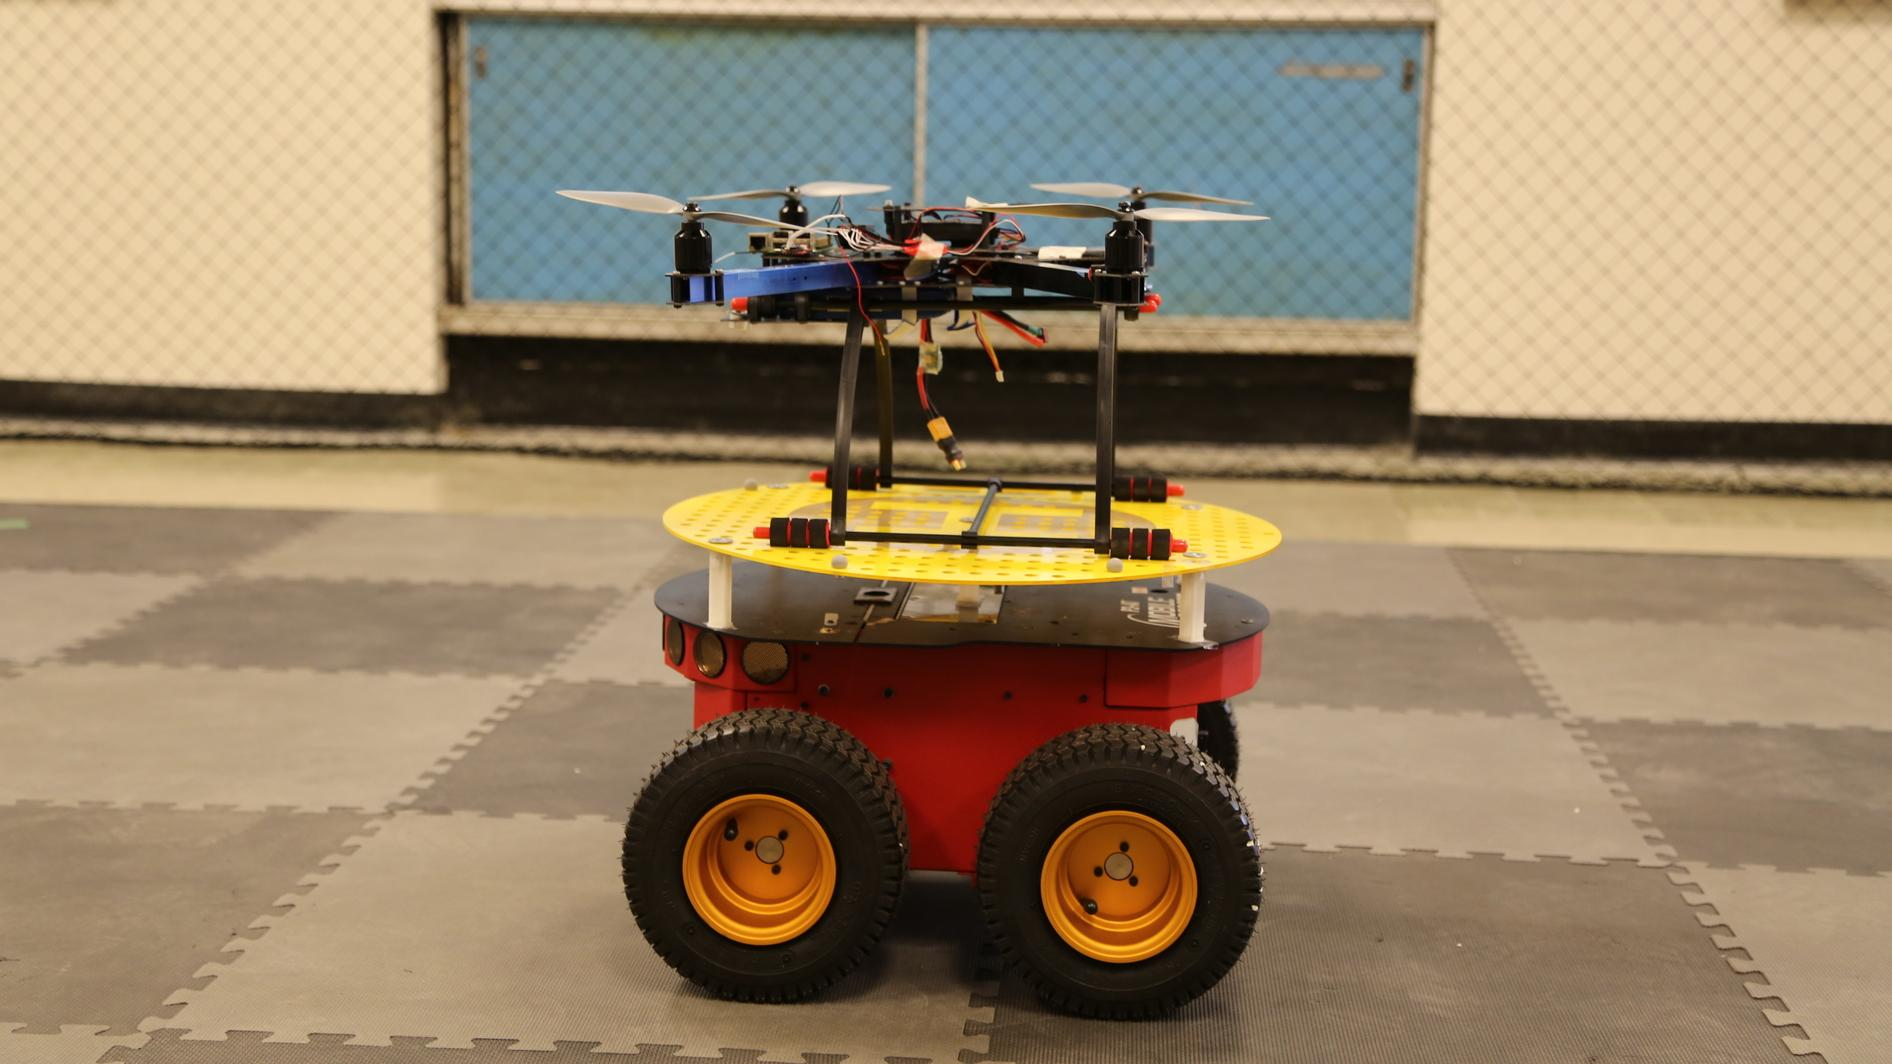
\includegraphics[width=0.6\textwidth]{images/irols.jpg}
    \caption{The test sUAV with the mobile target platform.}\label{f:lezl-olli}
\end{figure}

\subsection{Simulation}
Gazebo is a 3D simulation software which uses open source dynamics engines Bullet, Dart, and ODE to model its
components. While Gazebo has very high fidelity simulation capabilities for robots (its initial purpose), the
complexities of aerodynamics in general, and multicopter physics in particular, can only be modeled with many
simplifications. Even with the simplified dynamics, the simulation environment that Gazebo provides is very
useful for high-level controller development. Gazebo allows for the simulation of many sensor types and nicely
integrates with ROS and the PX4 flight controller firmware. The simulation
provides a real time interface for tuning the controller with visual feedback. This is the process which was
used to tune the fuzzy controller.

The most important aspect of sensing for the system is the image sensor. A camera sensor is simulated from the
underside of the quadrotor to test the efficacy and efficiency of the computer vision algorithms. Care was
taken to accurately represent the field of view and pixel noise of the physical camera sensor to be used.


\subsection{Onboard Software} ROS is an open source framework developed specifically to ease the development
of software for robotics and robotics control\cite{quigley2009ros}. Using ROS, it becomes a simple task to
distribute computational loads across a computational graph of separate nodes. Additionally, ROS has a rich
library of packages which are useful for both low-level processing of sensor information or managing hardware
interfaces, and also high-level behavioral control or localization schemes. This project use a number of such
packages to perform tasks in the areas of visual odometry\cite{olson2011tags}, kalman filtering
\cite{MooreStouchKeneralizedEkf2014}, and flight control\cite{rotors:2016,meier2015px4}. ROS allows for a
system designer to aggregate any number of processing units, called nodes, into a  complex computational graph.
An example of the graph structure created to complete this work is shown in \cref{f:rosgraph} and provides a
visualization of this complex structure. Each node in the graph represents a unit of computation which
consumes information from another node in the graph. Each edge in the graph represents a direct message
passing pipeline through which information is transmitted. Each node runs continuously and in parallel,
facilitating the creation of reactive, concurrent systems.

\begin{figure}[H]
    \centering
    \includedot[scale=0.29]{tikz/rosgraph_notf_cluster}
    \caption{Computational node graph for a typical landing simulation. Note that this graph may change over
    time as node may be dynamically started and stopped. Likewise, message passing pipelines may be opened or
    closed at any time.}\label{f:rosgraph}
\end{figure}

The nodes can be broadly categorized into three groups: Sensing nodes, Action states, and Control loop nodes.
The Sensing nodes consume image sensor output and pre-process it for Kalman filtering.
The Action states each represent a state in the state machine. These represent basic actions which the vehicle
can perform and can be aggregated to construct more complex behavior. The nodes in the Control loop represent
the plant (\verb|/mavros|), the sensor (\verb|/ekf_odom|), and the compensator (\verb|/flc_action|). In this
way, it becomes easy to visualize the canonical form of a feedback control loop. As can be seen in
\cref{f:rosgraph}, the structure allows a roboticist to build and manage highly complex systems in a
maintainable way.

\begin{figure}[H]
    \centering
    \includedot[scale=0.39]{tikz/smach}
    \caption{State machine of robotic lander}\label{f:smach}
\end{figure}

Control of the quadcopter is handled in discrete stages based on vehicle state. It is assumed that the vehicle
will have a rough estimate of the target location given to it so that it can travel to the appropriate region
and find the target in the field of view of the camera sensor. Vehicle motion from arming until target
location is handled by sending waypoints to the flight controller. Once the target is located in the image,
the vehicle gives control over to a set of FISs. The controller is described in more detail in
\cref{s:landing:controller}. The vehicle behavior over an entire mission is handled using a state
machine\cite{bohren2010smach}. Using a state machine allows the control to be handled in well-defined domains
and ensures that transitions between states are handled smoothly. The states comprising a full mission from
takeoff to landing are shown in \cref{f:smach}. A link to the video showing a full landing mission can be
found in the references section\cite{yt_stat}. An annotated image of the simulation at each state can be found
in \cref{app:smach} (example in \cref{f:sim_static_shot}).

\begin{figure}
    \centering
    \includegraphics[width=0.6\textwidth]{images/static_captures/static-15h39m54s115}
    \caption{Image of the simulation and live state diagram while vehicle is approaching the
    platform.}\label{f:sim_static_shot}
\end{figure}

The state of the vehicle is managed by fusing together the positional estimate from the camera sensor and the
AprilTag estimate (see \cref{s:landing:cv}), as well as orientation information from the onboard IMU using an
extended kalman filter (EKF). This estimate is only valid when the vehicle has a visual track on the target
platform; otherwise, it is assumed that the vehicle is still in transit from its launch location, or it has
landed. 

As can be seen in \cref{f:smach}, a mission starts in the ``ARM'' by arming the vehicle and immediately
sending it a waypoint which is near the target's location. Once the vehicle has received the waypoint, it
enters the ``TRACK'' state and is en route to the target location. While in this state, it monitors the
quality of its visual estimation of the target location by evaluating the norm of the covariance matrix 
computed by the EKF. Only when the covariance is sufficiently small does the vehicle transition to the next
state.

The transition to the ``APPROACH\_LAND'' state signals the transfer of control from the flight controller's
waypoint manager to the FISs. The "APPROACH\_LAND" state is simply a composition of two substates, "APPROACH"
and "LAND". During the "APPROACH" substate, the EKF is still running, sending estimates to the fuzzy logic
controller. The fuzzy logic controller is sending velocity setpoints to the onboard flight controller, thus
closing the feedback loop. The desired outcome of this state is to get the vehicle in a position above
the platform such that we can initiate the landing sequence. When the vehicle meets a proximity threshold,
it transitions to the ``LAND'' substate and puts down onto the landing pad. The details of the simulation,
control, vision estimation, and development process are discussed at length in the following sections.

\subsection{Computer Vision}\label{s:landing:cv}
Image processing is handled by a node in the ROS computation graph that is constantly processing image outputs
from the onboard camera. Once it senses the platform, it then publishes
a state estimation to the rest of the nodes in the ROS graph. Much emphasis is put on the sensing algorithms to be computationally efficient to decrease the load on the
on-board computer. For this purpose, only a small number of image processes are required to detect and locate
the target. As a first pass, the image is brought into the Hue-Saturation-Value (HSV) color space. This has
been shown to be a robust space in which to perform color detection and segmentation in uncontrolled and
unpredictable lighting conditions\cite{zhao2002robust}. A simple thresholding is performed on the image to
isolate a sufficiently wide band of yellows to match the color of the target and dilate this to a binary blob.
From this binary image, the image moments are calculated by
\begin{figure}[ht!]
    \centering
    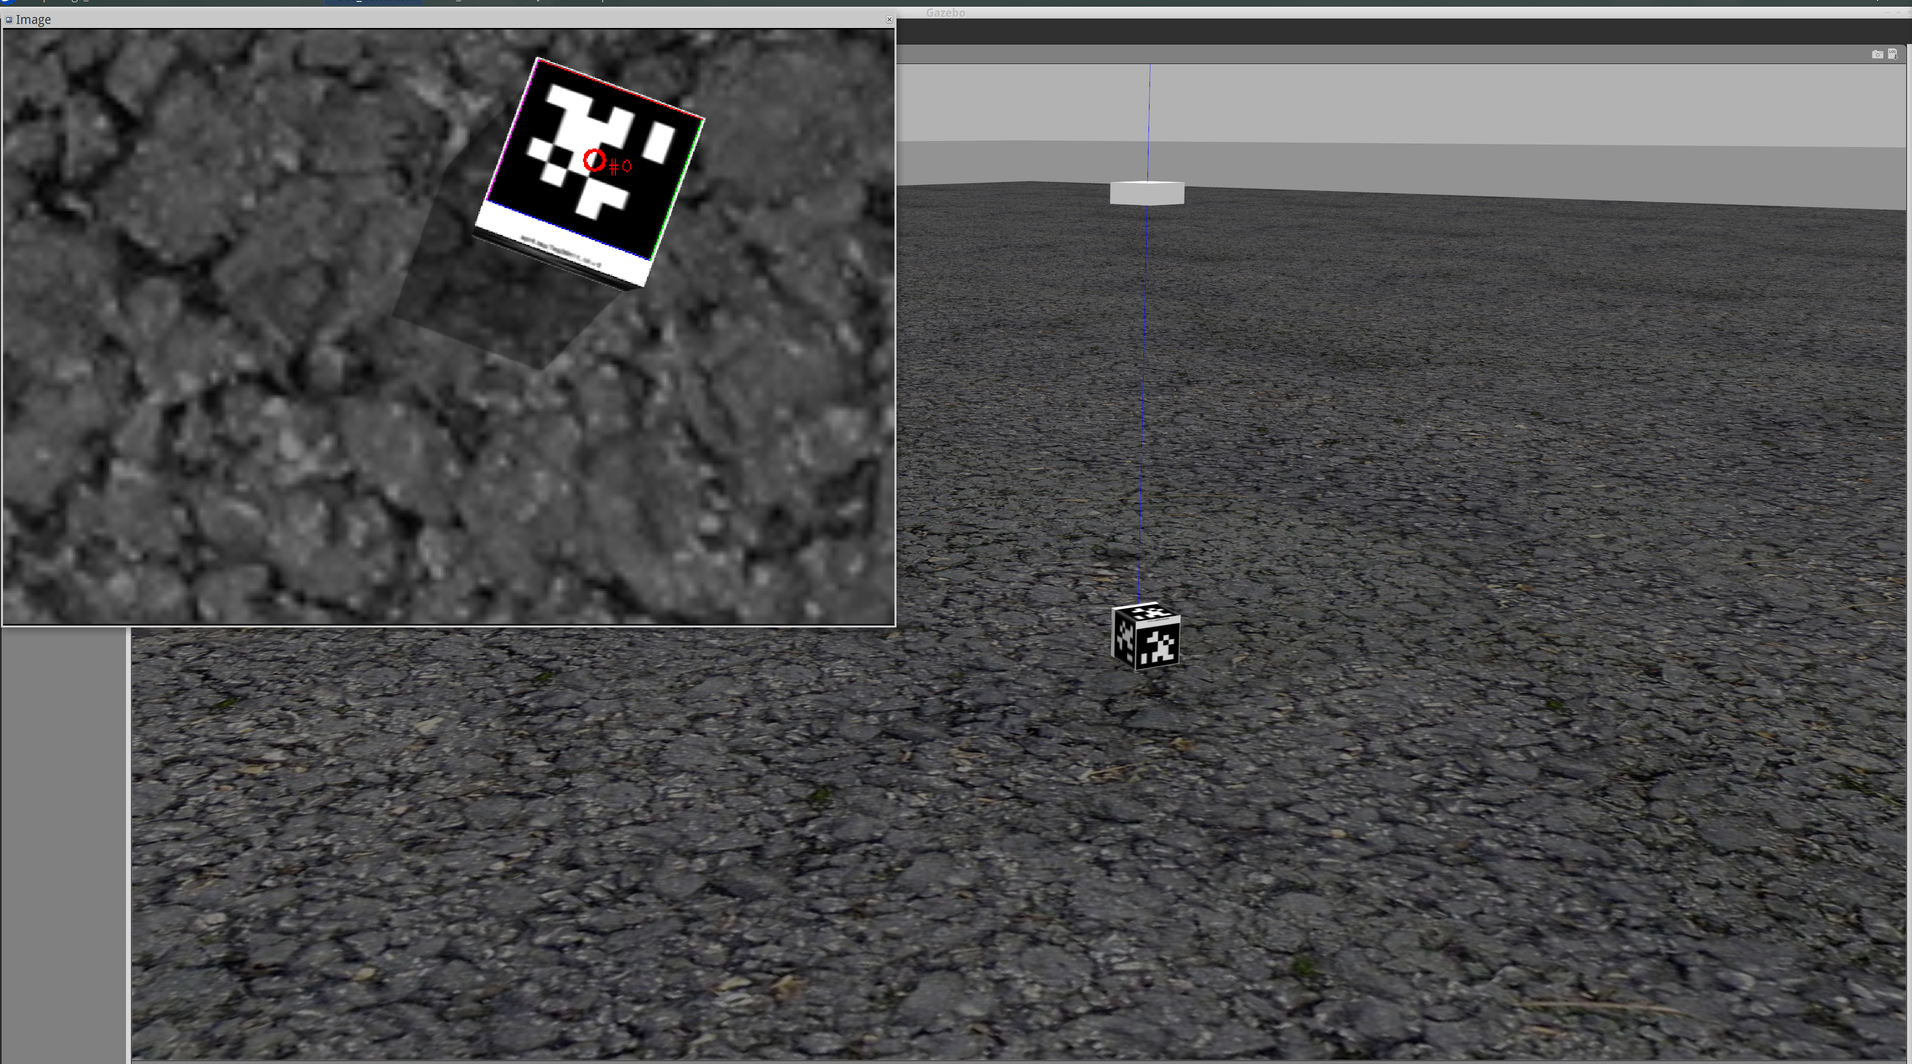
\includegraphics[width=0.8\textwidth]{images/rs_working_apriltags_crop.png}
    \caption{Simulated image sensor detection of AprilTag marker.}\label{f:apriltag}
\end{figure}

\begin{equation}\label{e:im_moments} 
    m_{ij}=\sum_{x,y}x^iy^jI_{xy}
\end{equation}
\nomenclature[]{$m_{ij}$}{Raw image moment}
\nomenclature[]{$I_{xy}$}{Pixel intensity value}
where $I_{xy}$ is the pixel intensity value for each pixel $(x,y)$ (equal to 1 for this binary blob) and $i,j
= 0,1,2$. From this it can be seen that $m_{00}$ describes the area and $\frac{m_{10}}{m_{00}}$ and
$\frac{m_{01}}{m_{00}}$ describe the centroids $\overline{x}_p$ and $\overline{y}_p$ in terms of
pixels\cite{hu1962visual}. The blob is assumed to be circular and hence a diameter is extracted from the pixel
area. Using the focal length of the sensor, these image points are then projected onto the ground plane using
the known diameter of the landing pad and a vertical offset estimate is obtained as is shown in
\cref{e:dist_est}.
\begin{equation}\label{e:dist_est}
    d_z=\frac{d\cdot f}{m\cdot d_p}
\end{equation}
where $f$ is the focal length of the camera in units of length, $d$ is the known diameter of the landing pad,
$d_p$ is the estimated diameter in pixels, and $m$ represents a scaling factor in units of \si{\px\per\mm}
(unity in the simulation).
\nomenclature[]{$f$}{Focal length of image sensor}
\nomenclature[]{$m$}{Pixel scaling factor}
Assuming that the image plane and the ground plane are parallel, the center of the image can be assumed to
point directly below the vehicle and the horizontal offsets to the landing pad can then be calculated as
\begin{align}\label{e:horiz_est}
    d_x &= d_z\cdot\frac{m\overline{x}_p}{f}\\
    d_y &= d_z\cdot\frac{m\overline{y}_p}{f}\label{e:horiz_est-y}
\end{align}
\nomenclature[]{$d_x$}{Horizontal offset error from vehicle to target in the body-fixed $x$-axis}
\nomenclature[]{$d_y$}{Horizontal offset error from vehicle to target in the body-fixed $y$-axis}
\nomenclature[]{$d_z$}{Vertical offset error from vehicle to the target}

Unless the camera is mounted to a perfect gimbal, the image plane cannot be assumed to be parallel to the
ground plane, thus invalidating \crefrange{e:horiz_est}{e:horiz_est-y}. To overcome this, the rotation
sequence needed to transform the image into body-relative coordinates is found and applied to the image data.
The camera is assumed to be rigidly affixed to the body of the vehicle, thus this is a simple static
transformation. Then, the vehicle body frame is related to the inertial frame by another rotation. The landing
pad is assumed to be on level ground and the distance between the vehicle and pad is estimated from
\cref{e:dist_est}. Note that although there will be image skew when the vehicle is under some rotation, the error in estimated distance this introduces is small compared to the actual distance of the vehicle from
the target. As the vehicle approaches the target, the estimate improves in quality due to a crisper image,
level flight, and the addition of AprilTag estimation.

In order to account for vehicle attitude, a rotation sequence is applied to the projected target location.
Let $R\left(\phi, \theta, \psi\right)$ be the rotation matrix defined as
\begin{equation}
    R(\phi,\theta,\psi) = 
    \begin{bmatrix}
            c_{\theta}c_{\psi}                           & -c_{\theta}s_{\phi}                           & s_{\theta}\\
            c_{\phi}s_{\psi} + c_{\psi}s_{\phi}s_{\theta} & c_{\phi}c_{\psi} - c_{\psi}s_{\phi}s_{\theta} & -c_{\theta}s_{\phi}\\
            s_{\phi}s_{\psi} -c_{\phi}c_{\psi}s_{\theta} & c_{\psi}s_{\phi} + c_{\phi}s_{\theta}s_{\psi} & c_{\phi}c_{\theta}
    \end{bmatrix}
\end{equation}
where $\phi$, $\theta$, and $\psi$ are vehicle roll, pitch and yaw respectively. $c_{\alpha}$ and $s_{\alpha}$
represent $\cos{\alpha}$ and $\sin{\alpha}$ respectively. Let $R_x^y$ represent the rotation from frame $x$ to
$y$, then $R_x^yR_y^z$ is the rotation from frame $x$ to frame $z$ with respect to the stationary frame $x$.
Now assuming the vehicle can estimate its orientation from the onboard inertial measurement unit, the
following rotation matrices can be defined.
\begin{align}
    R_{cam}^{body}   & = R(\pi, 0, 0)\label{e:rot_cam_bod}\\
    R_{body}^{inert} & = R(\phi, \theta, \psi)\label{e:rot_body_inert}
\end{align}
where $R_{x}^{y}$ represents the rotation from frame $x$ to frame $y$. These rotations are then prefixed to the
projected point found  in \crefrange{e:dist_est}{e:horiz_est-y} to find the point in world units with respect
to the vehicle.
\begin{align}\label{e:rotate}
    P_i = \begin{pmatrix}d_x\\d_y\\d_z\end{pmatrix}\\
    P_r = R_{body}^{inert}R_{cam}^{body}P_i
\end{align}
where $P_i$ is the projected point of the target in the plane parallel to the image plane, and $P_r$ is the
rotated point of the target with respect to the vehicle.

As the vehicle approaches the landing pad, the image field of view is overtaken by the landing pad itself and
the former segmentation no longer becomes effective. For this purpose, an AprilTag\cite{olson2011tags} (see
\cref{f:apriltag}) is placed on the center of the target. In \cref{f:landing_ims}, a landing approach is
illustrated from the viewpoint of the image sensor. This figure shows three different stages of the image
processing pipeline: raw image capture ( \crefrange{f:colora}{f:colorb}), AprilTag detection
(\crefrange{f:aprila}{f:aprilb}), and platform detection (\crefrange{f:cva}{f:cvb}). Individual estimates from
both the AprilTag detection and platform detection are then fused using an EKF (\cref{s:ekf}). 

\begin{figure}
    \begin{subfigmatrix}{4}% number of columns
        \subfigure[\label{f:colora}]{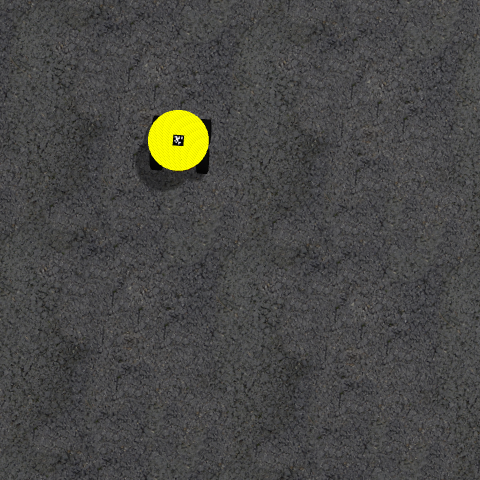
\includegraphics[width=0.2\textwidth]{images/image1_18469000.png}}
        \subfigure[]{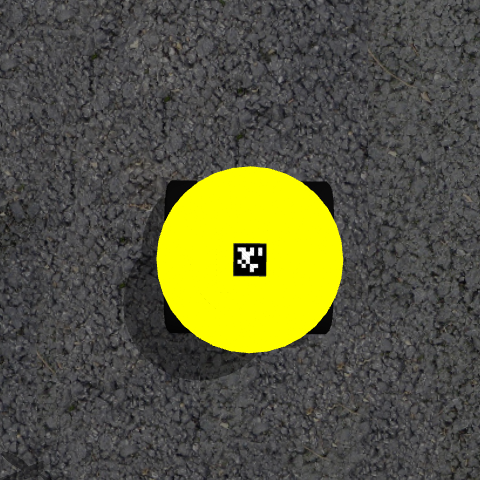
\includegraphics[width=0.2\textwidth]{images/image1_30863000.png}}
        \subfigure[]{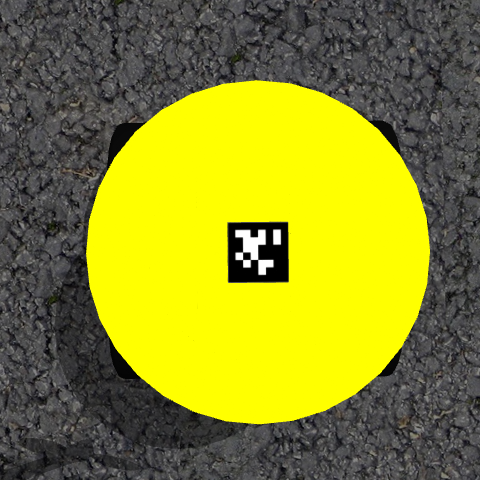
\includegraphics[width=0.2\textwidth]{images/image1_36074000.png}}
        \subfigure[\label{f:colorb}]{
\includegraphics[width=0.2\textwidth]{images/image1_38233000.png}}
        \subfigure[\label{f:aprila}]{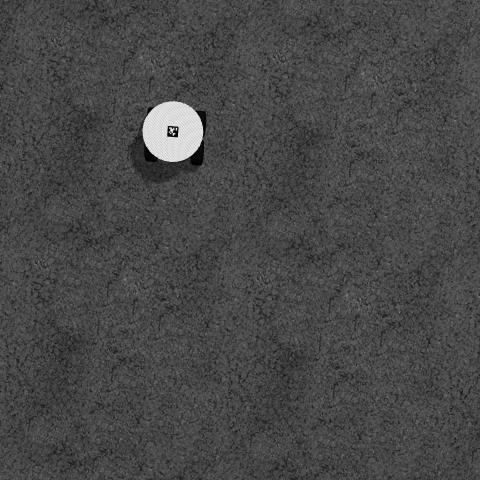
\includegraphics[width=0.2\textwidth]{images/image2_18469000.png}}
        \subfigure[]{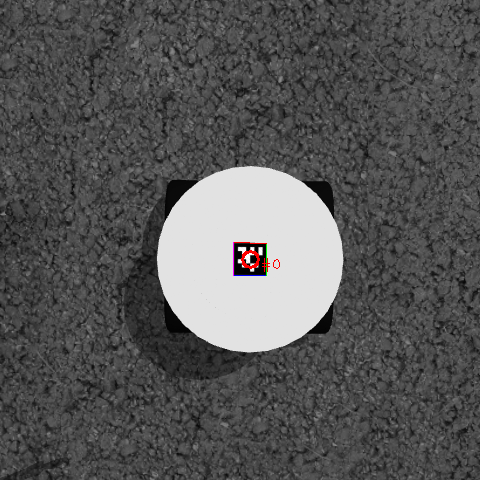
\includegraphics[width=0.2\textwidth]{images/image2_30863000.png}}
        \subfigure[]{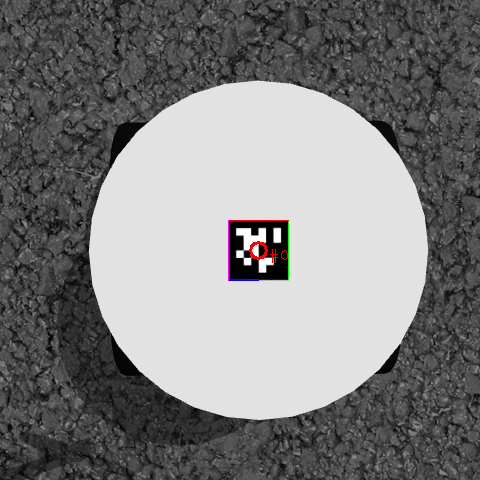
\includegraphics[width=0.2\textwidth]{images/image2_36074000.png}}
        \subfigure[\label{f:aprilb}]{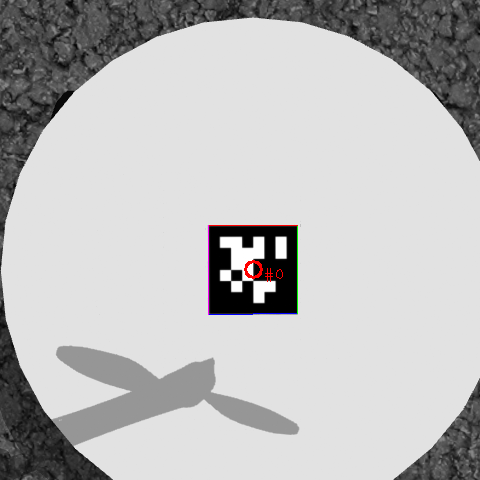
\includegraphics[width=0.2\textwidth]{images/image2_38233000.png}}
        \subfigure[\label{f:cva}]{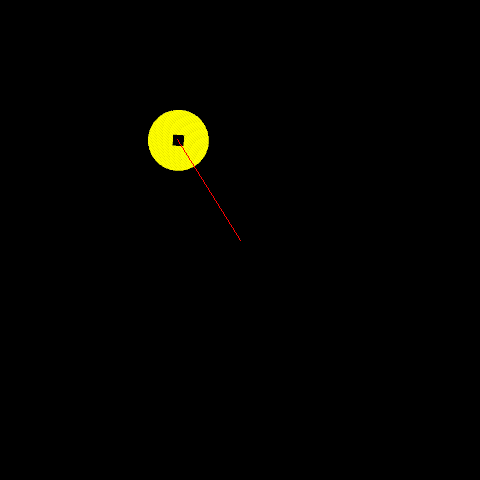
\includegraphics[width=0.2\textwidth]{images/image1_18469000_proc.png}}
        \subfigure[]{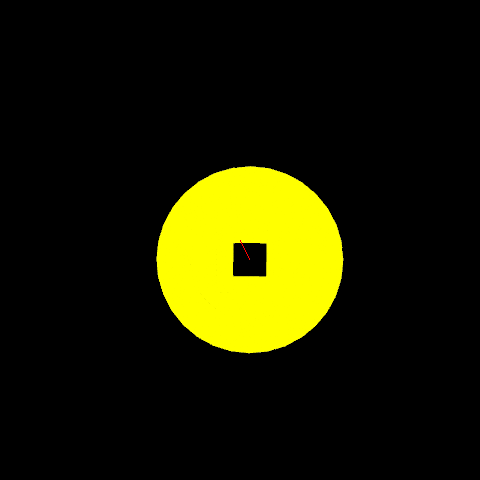
\includegraphics[width=0.2\textwidth]{images/image1_30863000_proc.png}}
        \subfigure[]{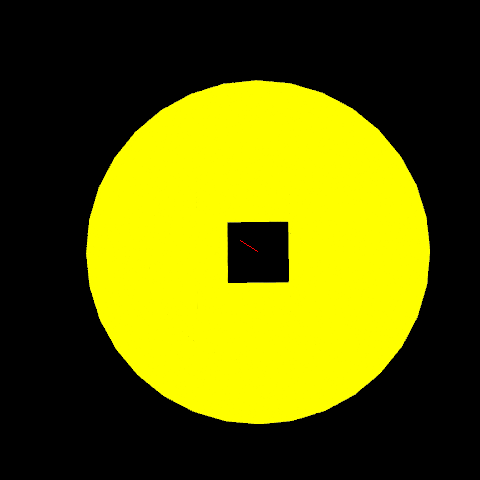
\includegraphics[width=0.2\textwidth]{images/image1_36074000_proc.png}}
        \subfigure[\label{f:cvb}]{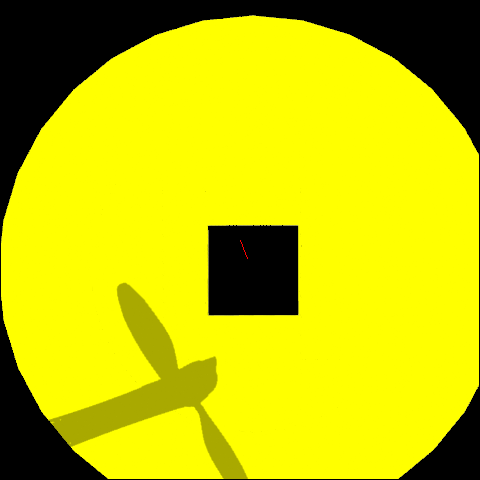
\includegraphics[width=0.2\textwidth]{images/image1_38233000_proc.png}}
    \end{subfigmatrix}
    \caption{A time series of images taken during the landing maneuver.}
    \label{f:landing_ims}
\end{figure}

\section{Controller}\label{s:landing:controller}
Control is actuated on the vehicle by providing velocity setpoints to the flight controller, $v_x$, $v_y$,
$v_z$, and yaw rate, $\dot{\psi}$. Ideally either linear acceleration setpoints or forces would be the control
output, but limitations in the flight controller make this impossible at this time. Setting velocities allows
the controller to cope with step changes to position offset well, but have difficulties tracking ramps. The
yaw angle, $\psi$ of the vehicle at landing is irrelevant for this project, but the controller is able to
control that axis regardless.

\subsection{PID Controller}
A PID controller was created which uses error estimates and sends velocity setpoints to the flight controller.
Due to the lack of a mathematical model of the system, the PID gains were found by iterating the simulation
with various position setpoints and dynamically adjusting the gains while observing the response visually.
This closely mimics the method by which PID gains are attained in the tuning of an actual quadrotor by flying
a series of test flights and adjusting gain values by feel. In this way, a reasonable response and landing
sequence was achieved for first a static target and then repeated for a dynamic target moving with constant
velocity. The results are presented in \crefrange{f:pid_stat}{f:pid_dyn} in which the normed horizontal offset
from target is shown in conjunction with the vertical distance to the platform. This view of the data gives an
overall sens of how the controller performs by showing how smooth the trajectory of the vehicle is as it
approaches the platform.  Viewing the charts, it is
apparent that as the vehicle approaches the target, it tends to accumulate horizontal errors and must correct
more frequently, particularly in the dynamic case. In both cases, the quadrotor managed to successfully land
on the target. In the static case, the final offset from the center of the target was less than \SI{5}{\cm}.
For the dynamic case, the error was \SI{7}{\cm} which nearly displaced it from the target surface. In both
cases, the sink rate and yaw rates were controlled by simple PD controllers. It can be seen that the controller took a significantly longer time to intercept and land
on the moving target as it repeatedly had trouble responding to the motion and would temporarily lose its
visual track. This is apparent in the large spiking errors in \cref{f:pid_dyn}.

%\begin{figure}
    %\centering
    %% GNUPLOT: LaTeX picture with Postscript
\begingroup
  \makeatletter
  \providecommand\color[2][]{%
    \GenericError{(gnuplot) \space\space\space\@spaces}{%
      Package color not loaded in conjunction with
      terminal option `colourtext'%
    }{See the gnuplot documentation for explanation.%
    }{Either use 'blacktext' in gnuplot or load the package
      color.sty in LaTeX.}%
    \renewcommand\color[2][]{}%
  }%
  \providecommand\includegraphics[2][]{%
    \GenericError{(gnuplot) \space\space\space\@spaces}{%
      Package graphicx or graphics not loaded%
    }{See the gnuplot documentation for explanation.%
    }{The gnuplot epslatex terminal needs graphicx.sty or graphics.sty.}%
    \renewcommand\includegraphics[2][]{}%
  }%
  \providecommand\rotatebox[2]{#2}%
  \@ifundefined{ifGPcolor}{%
    \newif\ifGPcolor
    \GPcolorfalse
  }{}%
  \@ifundefined{ifGPblacktext}{%
    \newif\ifGPblacktext
    \GPblacktexttrue
  }{}%
  % define a \g@addto@macro without @ in the name:
  \let\gplgaddtomacro\g@addto@macro
  % define empty templates for all commands taking text:
  \gdef\gplbacktext{}%
  \gdef\gplfronttext{}%
  \makeatother
  \ifGPblacktext
    % no textcolor at all
    \def\colorrgb#1{}%
    \def\colorgray#1{}%
  \else
    % gray or color?
    \ifGPcolor
      \def\colorrgb#1{\color[rgb]{#1}}%
      \def\colorgray#1{\color[gray]{#1}}%
      \expandafter\def\csname LTw\endcsname{\color{white}}%
      \expandafter\def\csname LTb\endcsname{\color{black}}%
      \expandafter\def\csname LTa\endcsname{\color{black}}%
      \expandafter\def\csname LT0\endcsname{\color[rgb]{1,0,0}}%
      \expandafter\def\csname LT1\endcsname{\color[rgb]{0,1,0}}%
      \expandafter\def\csname LT2\endcsname{\color[rgb]{0,0,1}}%
      \expandafter\def\csname LT3\endcsname{\color[rgb]{1,0,1}}%
      \expandafter\def\csname LT4\endcsname{\color[rgb]{0,1,1}}%
      \expandafter\def\csname LT5\endcsname{\color[rgb]{1,1,0}}%
      \expandafter\def\csname LT6\endcsname{\color[rgb]{0,0,0}}%
      \expandafter\def\csname LT7\endcsname{\color[rgb]{1,0.3,0}}%
      \expandafter\def\csname LT8\endcsname{\color[rgb]{0.5,0.5,0.5}}%
    \else
      % gray
      \def\colorrgb#1{\color{black}}%
      \def\colorgray#1{\color[gray]{#1}}%
      \expandafter\def\csname LTw\endcsname{\color{white}}%
      \expandafter\def\csname LTb\endcsname{\color{black}}%
      \expandafter\def\csname LTa\endcsname{\color{black}}%
      \expandafter\def\csname LT0\endcsname{\color{black}}%
      \expandafter\def\csname LT1\endcsname{\color{black}}%
      \expandafter\def\csname LT2\endcsname{\color{black}}%
      \expandafter\def\csname LT3\endcsname{\color{black}}%
      \expandafter\def\csname LT4\endcsname{\color{black}}%
      \expandafter\def\csname LT5\endcsname{\color{black}}%
      \expandafter\def\csname LT6\endcsname{\color{black}}%
      \expandafter\def\csname LT7\endcsname{\color{black}}%
      \expandafter\def\csname LT8\endcsname{\color{black}}%
    \fi
  \fi
    \setlength{\unitlength}{0.0500bp}%
    \ifx\gptboxheight\undefined%
      \newlength{\gptboxheight}%
      \newlength{\gptboxwidth}%
      \newsavebox{\gptboxtext}%
    \fi%
    \setlength{\fboxrule}{0.5pt}%
    \setlength{\fboxsep}{1pt}%
\begin{picture}(7200.00,5040.00)%
    \gplgaddtomacro\gplbacktext{%
      \csname LTb\endcsname%
      \put(946,704){\makebox(0,0)[r]{\strut{}$-0.5$}}%
      \csname LTb\endcsname%
      \put(946,1111){\makebox(0,0)[r]{\strut{}$0$}}%
      \csname LTb\endcsname%
      \put(946,1518){\makebox(0,0)[r]{\strut{}$0.5$}}%
      \csname LTb\endcsname%
      \put(946,1925){\makebox(0,0)[r]{\strut{}$1$}}%
      \csname LTb\endcsname%
      \put(946,2332){\makebox(0,0)[r]{\strut{}$1.5$}}%
      \csname LTb\endcsname%
      \put(946,2740){\makebox(0,0)[r]{\strut{}$2$}}%
      \csname LTb\endcsname%
      \put(946,3147){\makebox(0,0)[r]{\strut{}$2.5$}}%
      \csname LTb\endcsname%
      \put(946,3554){\makebox(0,0)[r]{\strut{}$3$}}%
      \csname LTb\endcsname%
      \put(946,3961){\makebox(0,0)[r]{\strut{}$3.5$}}%
      \csname LTb\endcsname%
      \put(946,4368){\makebox(0,0)[r]{\strut{}$4$}}%
      \csname LTb\endcsname%
      \put(946,4775){\makebox(0,0)[r]{\strut{}$4.5$}}%
      \csname LTb\endcsname%
      \put(1078,484){\makebox(0,0){\strut{}$0$}}%
      \csname LTb\endcsname%
      \put(1896,484){\makebox(0,0){\strut{}$5$}}%
      \csname LTb\endcsname%
      \put(2714,484){\makebox(0,0){\strut{}$10$}}%
      \csname LTb\endcsname%
      \put(3532,484){\makebox(0,0){\strut{}$15$}}%
      \csname LTb\endcsname%
      \put(4349,484){\makebox(0,0){\strut{}$20$}}%
      \csname LTb\endcsname%
      \put(5167,484){\makebox(0,0){\strut{}$25$}}%
      \csname LTb\endcsname%
      \put(5985,484){\makebox(0,0){\strut{}$30$}}%
      \csname LTb\endcsname%
      \put(6803,484){\makebox(0,0){\strut{}$35$}}%
    }%
    \gplgaddtomacro\gplfronttext{%
      \csname LTb\endcsname%
      \put(176,2739){\rotatebox{-270}{\makebox(0,0){\strut{}Error, m}}}%
      \put(3940,154){\makebox(0,0){\strut{}Time, s}}%
      \put(5816,4602){\makebox(0,0)[r]{\strut{}$e_{xy}$}}%
      \put(5816,4382){\makebox(0,0)[r]{\strut{}$e_z$}}%
    }%
    \gplbacktext
    \put(0,0){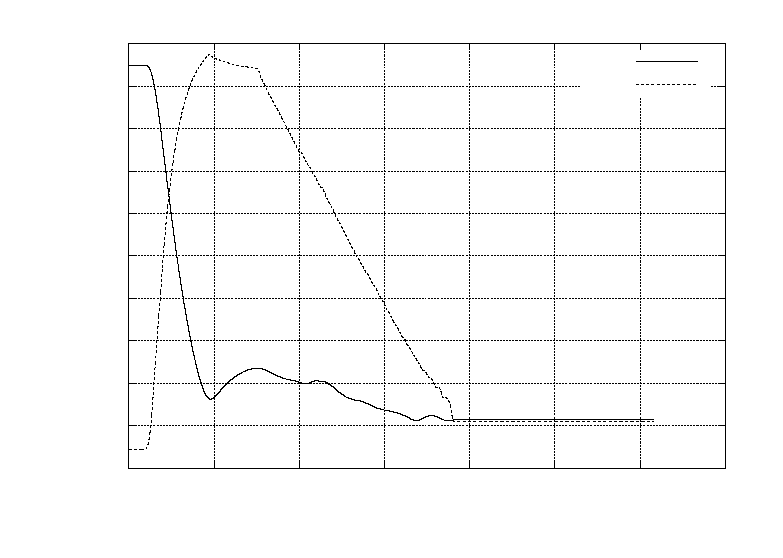
\includegraphics{static_smach_good_plot}}%
    \gplfronttext
  \end{picture}%
\endgroup

    %\caption{Fuzzy-controlled static target interception.}\label{f:fuz_stat}
%\end{figure}

%\begin{figure}
    %\centering
    %% GNUPLOT: LaTeX picture with Postscript
\begingroup
  \makeatletter
  \providecommand\color[2][]{%
    \GenericError{(gnuplot) \space\space\space\@spaces}{%
      Package color not loaded in conjunction with
      terminal option `colourtext'%
    }{See the gnuplot documentation for explanation.%
    }{Either use 'blacktext' in gnuplot or load the package
      color.sty in LaTeX.}%
    \renewcommand\color[2][]{}%
  }%
  \providecommand\includegraphics[2][]{%
    \GenericError{(gnuplot) \space\space\space\@spaces}{%
      Package graphicx or graphics not loaded%
    }{See the gnuplot documentation for explanation.%
    }{The gnuplot epslatex terminal needs graphicx.sty or graphics.sty.}%
    \renewcommand\includegraphics[2][]{}%
  }%
  \providecommand\rotatebox[2]{#2}%
  \@ifundefined{ifGPcolor}{%
    \newif\ifGPcolor
    \GPcolorfalse
  }{}%
  \@ifundefined{ifGPblacktext}{%
    \newif\ifGPblacktext
    \GPblacktexttrue
  }{}%
  % define a \g@addto@macro without @ in the name:
  \let\gplgaddtomacro\g@addto@macro
  % define empty templates for all commands taking text:
  \gdef\gplbacktext{}%
  \gdef\gplfronttext{}%
  \makeatother
  \ifGPblacktext
    % no textcolor at all
    \def\colorrgb#1{}%
    \def\colorgray#1{}%
  \else
    % gray or color?
    \ifGPcolor
      \def\colorrgb#1{\color[rgb]{#1}}%
      \def\colorgray#1{\color[gray]{#1}}%
      \expandafter\def\csname LTw\endcsname{\color{white}}%
      \expandafter\def\csname LTb\endcsname{\color{black}}%
      \expandafter\def\csname LTa\endcsname{\color{black}}%
      \expandafter\def\csname LT0\endcsname{\color[rgb]{1,0,0}}%
      \expandafter\def\csname LT1\endcsname{\color[rgb]{0,1,0}}%
      \expandafter\def\csname LT2\endcsname{\color[rgb]{0,0,1}}%
      \expandafter\def\csname LT3\endcsname{\color[rgb]{1,0,1}}%
      \expandafter\def\csname LT4\endcsname{\color[rgb]{0,1,1}}%
      \expandafter\def\csname LT5\endcsname{\color[rgb]{1,1,0}}%
      \expandafter\def\csname LT6\endcsname{\color[rgb]{0,0,0}}%
      \expandafter\def\csname LT7\endcsname{\color[rgb]{1,0.3,0}}%
      \expandafter\def\csname LT8\endcsname{\color[rgb]{0.5,0.5,0.5}}%
    \else
      % gray
      \def\colorrgb#1{\color{black}}%
      \def\colorgray#1{\color[gray]{#1}}%
      \expandafter\def\csname LTw\endcsname{\color{white}}%
      \expandafter\def\csname LTb\endcsname{\color{black}}%
      \expandafter\def\csname LTa\endcsname{\color{black}}%
      \expandafter\def\csname LT0\endcsname{\color{black}}%
      \expandafter\def\csname LT1\endcsname{\color{black}}%
      \expandafter\def\csname LT2\endcsname{\color{black}}%
      \expandafter\def\csname LT3\endcsname{\color{black}}%
      \expandafter\def\csname LT4\endcsname{\color{black}}%
      \expandafter\def\csname LT5\endcsname{\color{black}}%
      \expandafter\def\csname LT6\endcsname{\color{black}}%
      \expandafter\def\csname LT7\endcsname{\color{black}}%
      \expandafter\def\csname LT8\endcsname{\color{black}}%
    \fi
  \fi
    \setlength{\unitlength}{0.0500bp}%
    \ifx\gptboxheight\undefined%
      \newlength{\gptboxheight}%
      \newlength{\gptboxwidth}%
      \newsavebox{\gptboxtext}%
    \fi%
    \setlength{\fboxrule}{0.5pt}%
    \setlength{\fboxsep}{1pt}%
\begin{picture}(7200.00,5040.00)%
    \gplgaddtomacro\gplbacktext{%
      \csname LTb\endcsname%
      \put(682,704){\makebox(0,0)[r]{\strut{}$-1$}}%
      \csname LTb\endcsname%
      \put(682,1213){\makebox(0,0)[r]{\strut{}$0$}}%
      \csname LTb\endcsname%
      \put(682,1722){\makebox(0,0)[r]{\strut{}$1$}}%
      \csname LTb\endcsname%
      \put(682,2231){\makebox(0,0)[r]{\strut{}$2$}}%
      \csname LTb\endcsname%
      \put(682,2740){\makebox(0,0)[r]{\strut{}$3$}}%
      \csname LTb\endcsname%
      \put(682,3248){\makebox(0,0)[r]{\strut{}$4$}}%
      \csname LTb\endcsname%
      \put(682,3757){\makebox(0,0)[r]{\strut{}$5$}}%
      \csname LTb\endcsname%
      \put(682,4266){\makebox(0,0)[r]{\strut{}$6$}}%
      \csname LTb\endcsname%
      \put(682,4775){\makebox(0,0)[r]{\strut{}$7$}}%
      \csname LTb\endcsname%
      \put(814,484){\makebox(0,0){\strut{}$0$}}%
      \csname LTb\endcsname%
      \put(2012,484){\makebox(0,0){\strut{}$5$}}%
      \csname LTb\endcsname%
      \put(3210,484){\makebox(0,0){\strut{}$10$}}%
      \csname LTb\endcsname%
      \put(4407,484){\makebox(0,0){\strut{}$15$}}%
      \csname LTb\endcsname%
      \put(5605,484){\makebox(0,0){\strut{}$20$}}%
      \csname LTb\endcsname%
      \put(6803,484){\makebox(0,0){\strut{}$25$}}%
    }%
    \gplgaddtomacro\gplfronttext{%
      \csname LTb\endcsname%
      \put(176,2739){\rotatebox{-270}{\makebox(0,0){\strut{}Error, m}}}%
      \put(3808,154){\makebox(0,0){\strut{}Time, s}}%
      \put(5816,4602){\makebox(0,0)[r]{\strut{}$e_{xy}$}}%
      \put(5816,4382){\makebox(0,0)[r]{\strut{}$e_z$}}%
    }%
    \gplbacktext
    \put(0,0){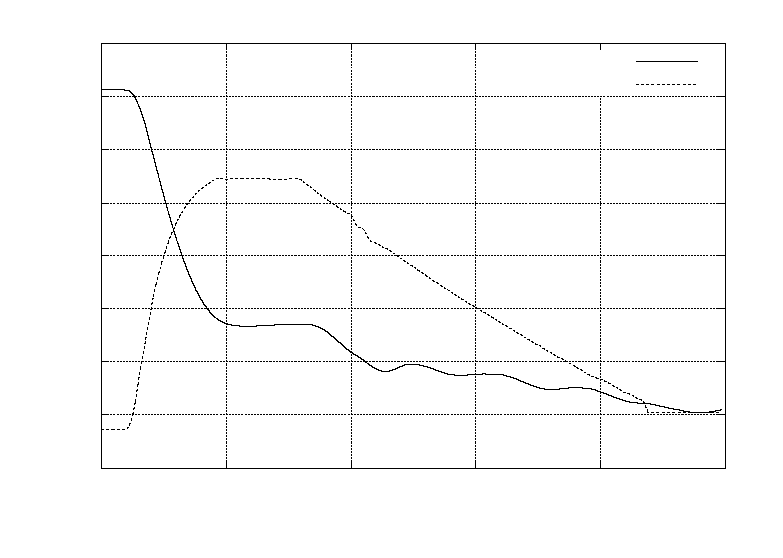
\includegraphics{moving_line_good_plot}}%
    \gplfronttext
  \end{picture}%
\endgroup

    %\caption{Fuzzy-controlled dynamic target interception.}\label{f:fuz_dyn}
%\end{figure}

\begin{figure}
    \centering
    % GNUPLOT: LaTeX picture with Postscript
\begingroup
  \makeatletter
  \providecommand\color[2][]{%
    \GenericError{(gnuplot) \space\space\space\@spaces}{%
      Package color not loaded in conjunction with
      terminal option `colourtext'%
    }{See the gnuplot documentation for explanation.%
    }{Either use 'blacktext' in gnuplot or load the package
      color.sty in LaTeX.}%
    \renewcommand\color[2][]{}%
  }%
  \providecommand\includegraphics[2][]{%
    \GenericError{(gnuplot) \space\space\space\@spaces}{%
      Package graphicx or graphics not loaded%
    }{See the gnuplot documentation for explanation.%
    }{The gnuplot epslatex terminal needs graphicx.sty or graphics.sty.}%
    \renewcommand\includegraphics[2][]{}%
  }%
  \providecommand\rotatebox[2]{#2}%
  \@ifundefined{ifGPcolor}{%
    \newif\ifGPcolor
    \GPcolorfalse
  }{}%
  \@ifundefined{ifGPblacktext}{%
    \newif\ifGPblacktext
    \GPblacktexttrue
  }{}%
  % define a \g@addto@macro without @ in the name:
  \let\gplgaddtomacro\g@addto@macro
  % define empty templates for all commands taking text:
  \gdef\gplbacktext{}%
  \gdef\gplfronttext{}%
  \makeatother
  \ifGPblacktext
    % no textcolor at all
    \def\colorrgb#1{}%
    \def\colorgray#1{}%
  \else
    % gray or color?
    \ifGPcolor
      \def\colorrgb#1{\color[rgb]{#1}}%
      \def\colorgray#1{\color[gray]{#1}}%
      \expandafter\def\csname LTw\endcsname{\color{white}}%
      \expandafter\def\csname LTb\endcsname{\color{black}}%
      \expandafter\def\csname LTa\endcsname{\color{black}}%
      \expandafter\def\csname LT0\endcsname{\color[rgb]{1,0,0}}%
      \expandafter\def\csname LT1\endcsname{\color[rgb]{0,1,0}}%
      \expandafter\def\csname LT2\endcsname{\color[rgb]{0,0,1}}%
      \expandafter\def\csname LT3\endcsname{\color[rgb]{1,0,1}}%
      \expandafter\def\csname LT4\endcsname{\color[rgb]{0,1,1}}%
      \expandafter\def\csname LT5\endcsname{\color[rgb]{1,1,0}}%
      \expandafter\def\csname LT6\endcsname{\color[rgb]{0,0,0}}%
      \expandafter\def\csname LT7\endcsname{\color[rgb]{1,0.3,0}}%
      \expandafter\def\csname LT8\endcsname{\color[rgb]{0.5,0.5,0.5}}%
    \else
      % gray
      \def\colorrgb#1{\color{black}}%
      \def\colorgray#1{\color[gray]{#1}}%
      \expandafter\def\csname LTw\endcsname{\color{white}}%
      \expandafter\def\csname LTb\endcsname{\color{black}}%
      \expandafter\def\csname LTa\endcsname{\color{black}}%
      \expandafter\def\csname LT0\endcsname{\color{black}}%
      \expandafter\def\csname LT1\endcsname{\color{black}}%
      \expandafter\def\csname LT2\endcsname{\color{black}}%
      \expandafter\def\csname LT3\endcsname{\color{black}}%
      \expandafter\def\csname LT4\endcsname{\color{black}}%
      \expandafter\def\csname LT5\endcsname{\color{black}}%
      \expandafter\def\csname LT6\endcsname{\color{black}}%
      \expandafter\def\csname LT7\endcsname{\color{black}}%
      \expandafter\def\csname LT8\endcsname{\color{black}}%
    \fi
  \fi
    \setlength{\unitlength}{0.0500bp}%
    \ifx\gptboxheight\undefined%
      \newlength{\gptboxheight}%
      \newlength{\gptboxwidth}%
      \newsavebox{\gptboxtext}%
    \fi%
    \setlength{\fboxrule}{0.5pt}%
    \setlength{\fboxsep}{1pt}%
\begin{picture}(7200.00,5040.00)%
    \gplgaddtomacro\gplbacktext{%
      \csname LTb\endcsname%
      \put(682,704){\makebox(0,0)[r]{\strut{}$-1$}}%
      \csname LTb\endcsname%
      \put(682,1213){\makebox(0,0)[r]{\strut{}$0$}}%
      \csname LTb\endcsname%
      \put(682,1722){\makebox(0,0)[r]{\strut{}$1$}}%
      \csname LTb\endcsname%
      \put(682,2231){\makebox(0,0)[r]{\strut{}$2$}}%
      \csname LTb\endcsname%
      \put(682,2740){\makebox(0,0)[r]{\strut{}$3$}}%
      \csname LTb\endcsname%
      \put(682,3248){\makebox(0,0)[r]{\strut{}$4$}}%
      \csname LTb\endcsname%
      \put(682,3757){\makebox(0,0)[r]{\strut{}$5$}}%
      \csname LTb\endcsname%
      \put(682,4266){\makebox(0,0)[r]{\strut{}$6$}}%
      \csname LTb\endcsname%
      \put(682,4775){\makebox(0,0)[r]{\strut{}$7$}}%
      \csname LTb\endcsname%
      \put(814,484){\makebox(0,0){\strut{}$15$}}%
      \csname LTb\endcsname%
      \put(1479,484){\makebox(0,0){\strut{}$20$}}%
      \csname LTb\endcsname%
      \put(2145,484){\makebox(0,0){\strut{}$25$}}%
      \csname LTb\endcsname%
      \put(2810,484){\makebox(0,0){\strut{}$30$}}%
      \csname LTb\endcsname%
      \put(3476,484){\makebox(0,0){\strut{}$35$}}%
      \csname LTb\endcsname%
      \put(4141,484){\makebox(0,0){\strut{}$40$}}%
      \csname LTb\endcsname%
      \put(4807,484){\makebox(0,0){\strut{}$45$}}%
      \csname LTb\endcsname%
      \put(5472,484){\makebox(0,0){\strut{}$50$}}%
      \csname LTb\endcsname%
      \put(6138,484){\makebox(0,0){\strut{}$55$}}%
      \csname LTb\endcsname%
      \put(6803,484){\makebox(0,0){\strut{}$60$}}%
    }%
    \gplgaddtomacro\gplfronttext{%
      \csname LTb\endcsname%
      \put(176,2739){\rotatebox{-270}{\makebox(0,0){\strut{}Error, m}}}%
      \put(3808,154){\makebox(0,0){\strut{}Time, s}}%
      \put(5816,4602){\makebox(0,0)[r]{\strut{}$e_{xy}$}}%
      \put(5816,4382){\makebox(0,0)[r]{\strut{}$e_z$}}%
    }%
    \gplbacktext
    \put(0,0){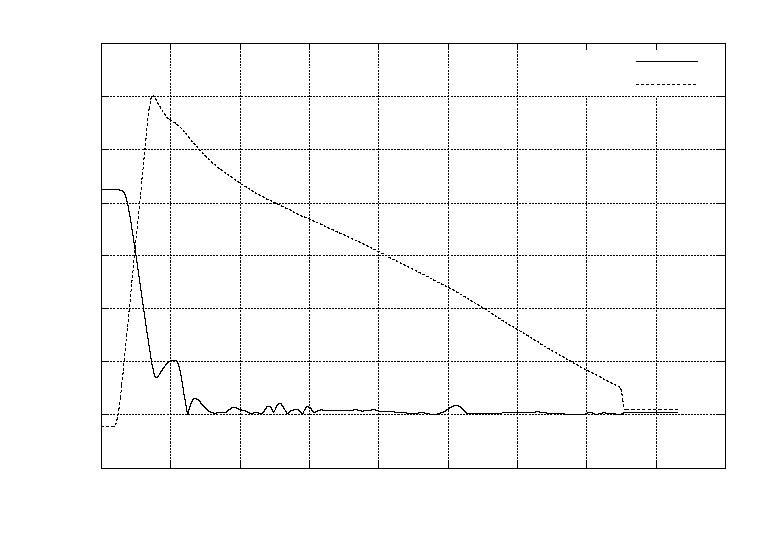
\includegraphics{pid_static}}%
    \gplfronttext
  \end{picture}%
\endgroup

    %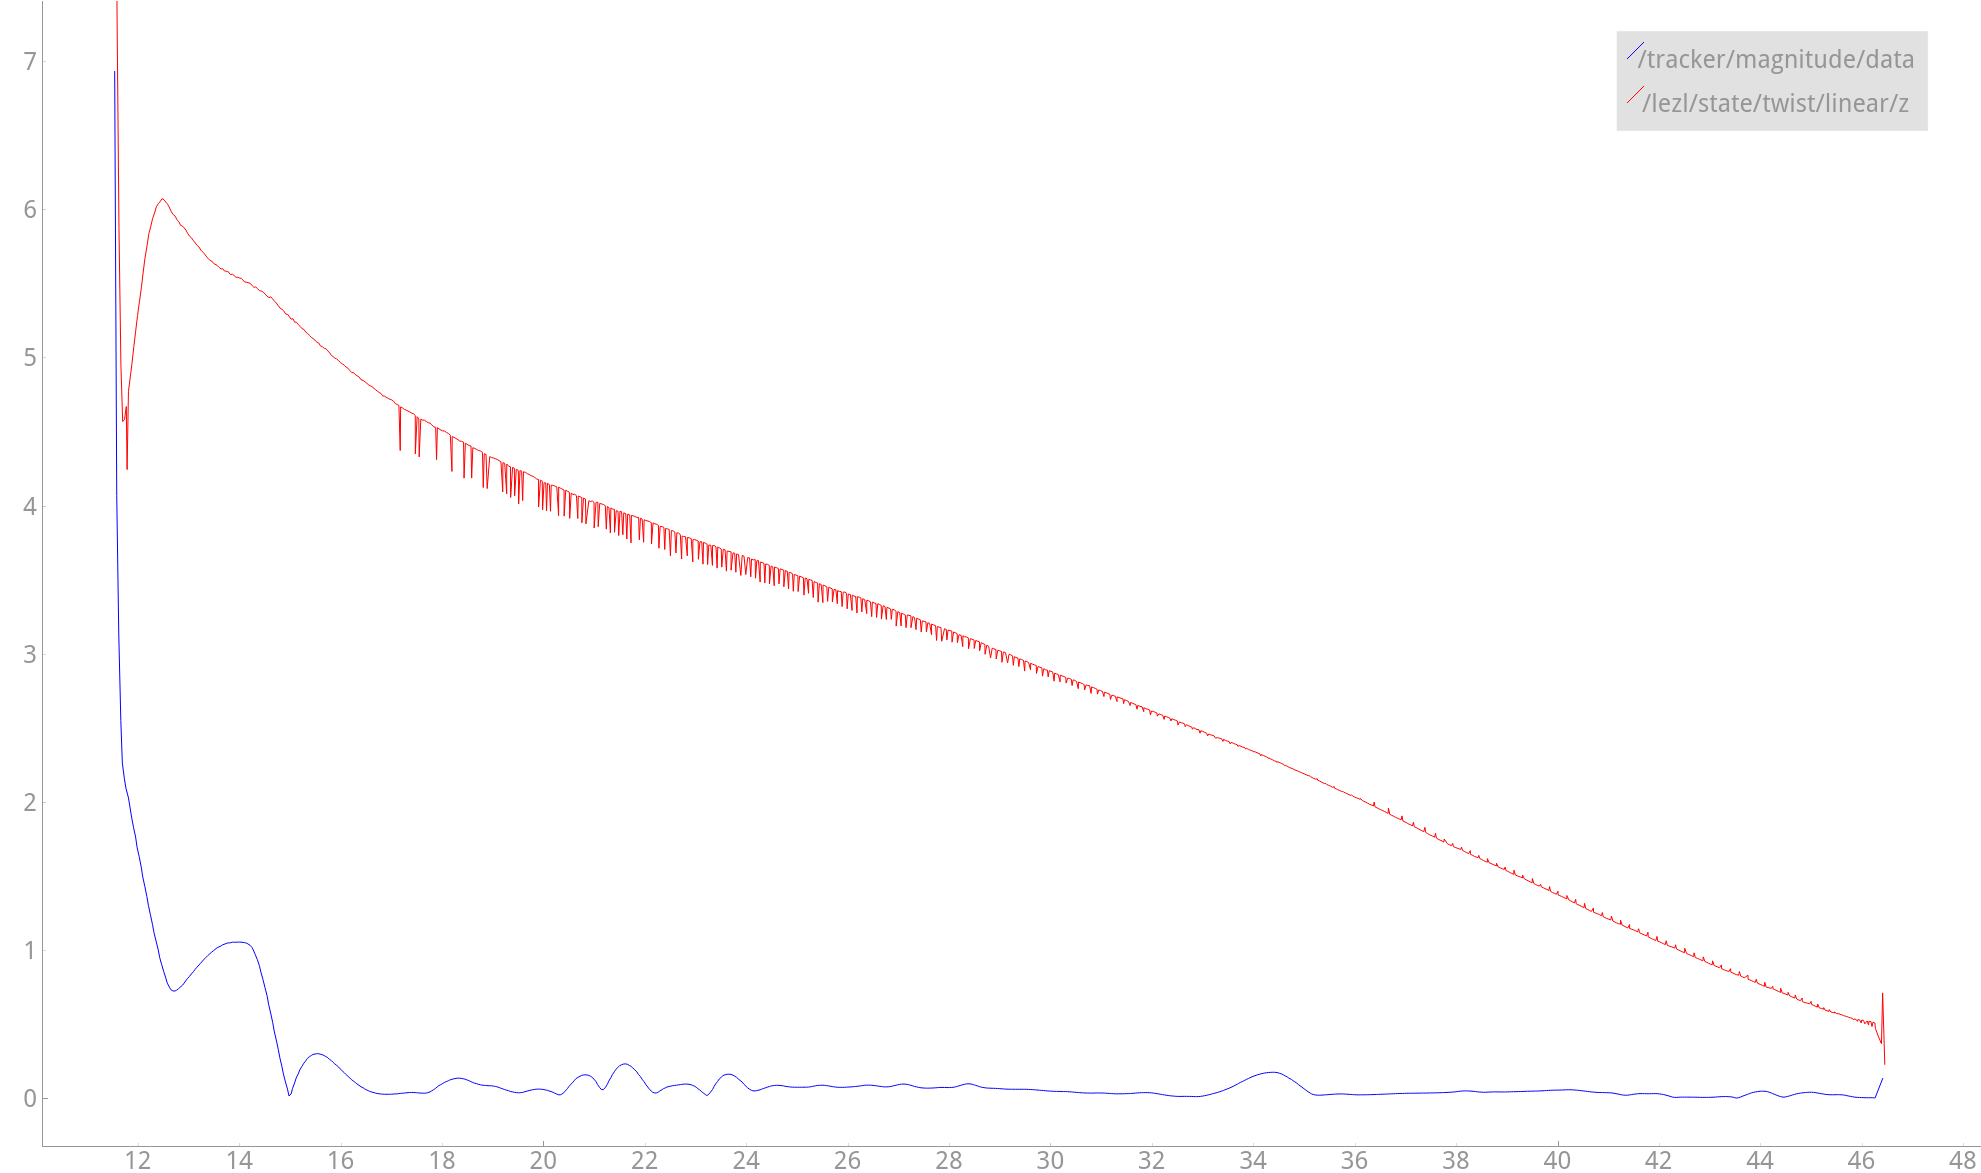
\includegraphics[width=0.9\textwidth]{images/mag_z_pid_static.png}
    \caption{$(kp,ki,kd)=(2.1,0.015,0.2)$ for static target interception.}\label{f:pid_stat}
\end{figure}

\begin{figure}
    \centering
    % GNUPLOT: LaTeX picture with Postscript
\begingroup
  \makeatletter
  \providecommand\color[2][]{%
    \GenericError{(gnuplot) \space\space\space\@spaces}{%
      Package color not loaded in conjunction with
      terminal option `colourtext'%
    }{See the gnuplot documentation for explanation.%
    }{Either use 'blacktext' in gnuplot or load the package
      color.sty in LaTeX.}%
    \renewcommand\color[2][]{}%
  }%
  \providecommand\includegraphics[2][]{%
    \GenericError{(gnuplot) \space\space\space\@spaces}{%
      Package graphicx or graphics not loaded%
    }{See the gnuplot documentation for explanation.%
    }{The gnuplot epslatex terminal needs graphicx.sty or graphics.sty.}%
    \renewcommand\includegraphics[2][]{}%
  }%
  \providecommand\rotatebox[2]{#2}%
  \@ifundefined{ifGPcolor}{%
    \newif\ifGPcolor
    \GPcolorfalse
  }{}%
  \@ifundefined{ifGPblacktext}{%
    \newif\ifGPblacktext
    \GPblacktexttrue
  }{}%
  % define a \g@addto@macro without @ in the name:
  \let\gplgaddtomacro\g@addto@macro
  % define empty templates for all commands taking text:
  \gdef\gplbacktext{}%
  \gdef\gplfronttext{}%
  \makeatother
  \ifGPblacktext
    % no textcolor at all
    \def\colorrgb#1{}%
    \def\colorgray#1{}%
  \else
    % gray or color?
    \ifGPcolor
      \def\colorrgb#1{\color[rgb]{#1}}%
      \def\colorgray#1{\color[gray]{#1}}%
      \expandafter\def\csname LTw\endcsname{\color{white}}%
      \expandafter\def\csname LTb\endcsname{\color{black}}%
      \expandafter\def\csname LTa\endcsname{\color{black}}%
      \expandafter\def\csname LT0\endcsname{\color[rgb]{1,0,0}}%
      \expandafter\def\csname LT1\endcsname{\color[rgb]{0,1,0}}%
      \expandafter\def\csname LT2\endcsname{\color[rgb]{0,0,1}}%
      \expandafter\def\csname LT3\endcsname{\color[rgb]{1,0,1}}%
      \expandafter\def\csname LT4\endcsname{\color[rgb]{0,1,1}}%
      \expandafter\def\csname LT5\endcsname{\color[rgb]{1,1,0}}%
      \expandafter\def\csname LT6\endcsname{\color[rgb]{0,0,0}}%
      \expandafter\def\csname LT7\endcsname{\color[rgb]{1,0.3,0}}%
      \expandafter\def\csname LT8\endcsname{\color[rgb]{0.5,0.5,0.5}}%
    \else
      % gray
      \def\colorrgb#1{\color{black}}%
      \def\colorgray#1{\color[gray]{#1}}%
      \expandafter\def\csname LTw\endcsname{\color{white}}%
      \expandafter\def\csname LTb\endcsname{\color{black}}%
      \expandafter\def\csname LTa\endcsname{\color{black}}%
      \expandafter\def\csname LT0\endcsname{\color{black}}%
      \expandafter\def\csname LT1\endcsname{\color{black}}%
      \expandafter\def\csname LT2\endcsname{\color{black}}%
      \expandafter\def\csname LT3\endcsname{\color{black}}%
      \expandafter\def\csname LT4\endcsname{\color{black}}%
      \expandafter\def\csname LT5\endcsname{\color{black}}%
      \expandafter\def\csname LT6\endcsname{\color{black}}%
      \expandafter\def\csname LT7\endcsname{\color{black}}%
      \expandafter\def\csname LT8\endcsname{\color{black}}%
    \fi
  \fi
    \setlength{\unitlength}{0.0500bp}%
    \ifx\gptboxheight\undefined%
      \newlength{\gptboxheight}%
      \newlength{\gptboxwidth}%
      \newsavebox{\gptboxtext}%
    \fi%
    \setlength{\fboxrule}{0.5pt}%
    \setlength{\fboxsep}{1pt}%
\begin{picture}(7200.00,5040.00)%
    \gplgaddtomacro\gplbacktext{%
      \csname LTb\endcsname%
      \put(682,704){\makebox(0,0)[r]{\strut{}$0$}}%
      \csname LTb\endcsname%
      \put(682,1111){\makebox(0,0)[r]{\strut{}$1$}}%
      \csname LTb\endcsname%
      \put(682,1518){\makebox(0,0)[r]{\strut{}$2$}}%
      \csname LTb\endcsname%
      \put(682,1925){\makebox(0,0)[r]{\strut{}$3$}}%
      \csname LTb\endcsname%
      \put(682,2332){\makebox(0,0)[r]{\strut{}$4$}}%
      \csname LTb\endcsname%
      \put(682,2740){\makebox(0,0)[r]{\strut{}$5$}}%
      \csname LTb\endcsname%
      \put(682,3147){\makebox(0,0)[r]{\strut{}$6$}}%
      \csname LTb\endcsname%
      \put(682,3554){\makebox(0,0)[r]{\strut{}$7$}}%
      \csname LTb\endcsname%
      \put(682,3961){\makebox(0,0)[r]{\strut{}$8$}}%
      \csname LTb\endcsname%
      \put(682,4368){\makebox(0,0)[r]{\strut{}$9$}}%
      \csname LTb\endcsname%
      \put(682,4775){\makebox(0,0)[r]{\strut{}$10$}}%
      \csname LTb\endcsname%
      \put(814,484){\makebox(0,0){\strut{}$10$}}%
      \csname LTb\endcsname%
      \put(1479,484){\makebox(0,0){\strut{}$15$}}%
      \csname LTb\endcsname%
      \put(2145,484){\makebox(0,0){\strut{}$20$}}%
      \csname LTb\endcsname%
      \put(2810,484){\makebox(0,0){\strut{}$25$}}%
      \csname LTb\endcsname%
      \put(3476,484){\makebox(0,0){\strut{}$30$}}%
      \csname LTb\endcsname%
      \put(4141,484){\makebox(0,0){\strut{}$35$}}%
      \csname LTb\endcsname%
      \put(4807,484){\makebox(0,0){\strut{}$40$}}%
      \csname LTb\endcsname%
      \put(5472,484){\makebox(0,0){\strut{}$45$}}%
      \csname LTb\endcsname%
      \put(6138,484){\makebox(0,0){\strut{}$50$}}%
      \csname LTb\endcsname%
      \put(6803,484){\makebox(0,0){\strut{}$55$}}%
    }%
    \gplgaddtomacro\gplfronttext{%
      \csname LTb\endcsname%
      \put(176,2739){\rotatebox{-270}{\makebox(0,0){\strut{}Error, m}}}%
      \put(3808,154){\makebox(0,0){\strut{}Time, s}}%
      \put(5816,4602){\makebox(0,0)[r]{\strut{}$e_{xy}$}}%
      \put(5816,4382){\makebox(0,0)[r]{\strut{}$e_z$}}%
    }%
    \gplbacktext
    \put(0,0){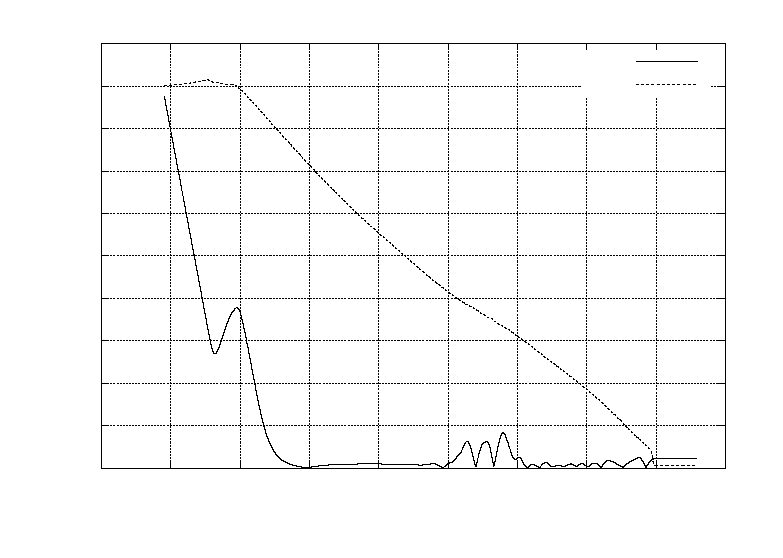
\includegraphics{pid_dyn}}%
    \gplfronttext
  \end{picture}%
\endgroup

    %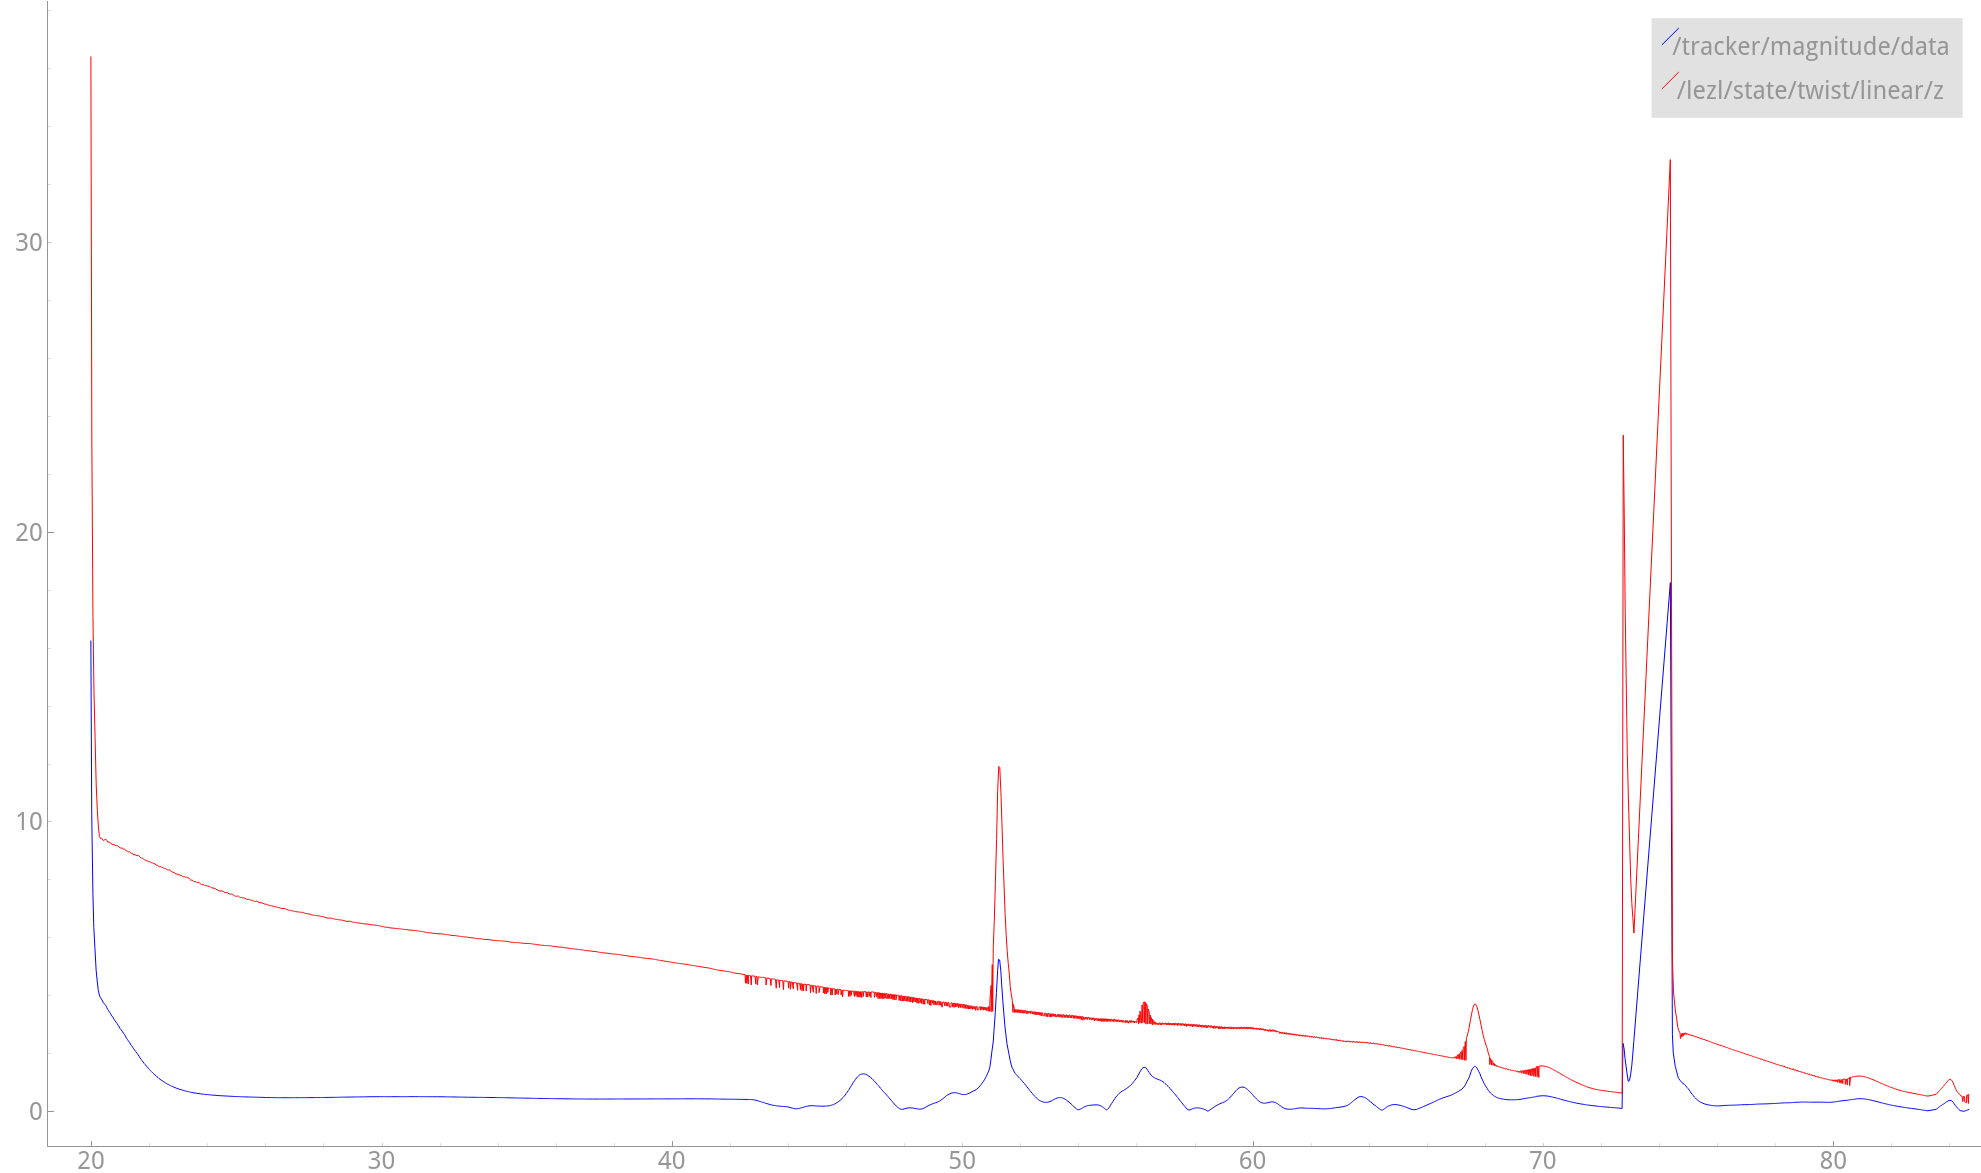
\includegraphics[width=0.9\textwidth]{images/mag_z_pid_dynamic.png}
    \caption{$(k_p,k_i,k_d)=(1.8,0.012,0.02)$ for dynamic target interception. The target is moving with a
    velocity of \SI{0.1}{\meter\per\s} in a straight line.}\label{f:pid_dyn}
\end{figure}


\subsection{Kalman Filter}\label{s:ekf}
In order to reduce the deleterious effect of instantaneous error accumulation when losing a visual track, a
kalman filter is introduced.  The filter provides a continuous, fused estimate of the vehicle's position
relative to the platform whenever there is at least visual sensing of the platform. This is done using the
\verb|robot_localization| package from ROS\cite{MooreStouchKeneralizedEkf2014}. This package is an
implementation of an extended kalman filter (EKF). The EKF provides a means by which to predict the vehicle
state even in the absence of current measurement\cite{kalman1960new}. The prediction is then corrected when
new measurement values are obtained. The measurements used to update the filter state are 1) the estimate from
the computer vision algorithm to update the vehicle position, 2) the estimate from the
AprilTag\cite{olson2011tags} routine to update both position and orientation, and 3) the IMU to
update angular rates and linear accelerations. These measurements are fused together to build an internal
model estimate of the dynamics of the vehicle. It is this model which provides the predictions between
measurements. An example of the EKF measurement is shown in \cref{f:ekf_plot}. It can be seen in this data
that though the visual estimate is very noisy, the EKF fusion follows the truth signal closely even between
the infrequent update periods of the accurate AprilTag measurement.

\begin{figure}[ht]
    \centering
    \begin{tikzpicture}[gnuplot]
%% generated with GNUPLOT 5.0p3 (Lua 5.1; terminal rev. 99, script rev. 100)
%% Mon 26 Mar 2018 04:08:56 AM EDT
\path (0.000,0.000) rectangle (12.500,8.750);
\gpcolor{color=gp lt color border}
\gpsetlinetype{gp lt border}
\gpsetdashtype{gp dt solid}
\gpsetlinewidth{1.00}
\draw[gp path] (1.504,0.985)--(1.684,0.985);
\draw[gp path] (11.947,0.985)--(11.767,0.985);
\node[gp node right] at (1.320,0.985) {$0$};
\draw[gp path] (1.504,1.807)--(1.684,1.807);
\draw[gp path] (11.947,1.807)--(11.767,1.807);
\node[gp node right] at (1.320,1.807) {$0.01$};
\draw[gp path] (1.504,2.629)--(1.684,2.629);
\draw[gp path] (11.947,2.629)--(11.767,2.629);
\node[gp node right] at (1.320,2.629) {$0.02$};
\draw[gp path] (1.504,3.450)--(1.684,3.450);
\draw[gp path] (11.947,3.450)--(11.767,3.450);
\node[gp node right] at (1.320,3.450) {$0.03$};
\draw[gp path] (1.504,4.272)--(1.684,4.272);
\draw[gp path] (11.947,4.272)--(11.767,4.272);
\node[gp node right] at (1.320,4.272) {$0.04$};
\draw[gp path] (1.504,5.094)--(1.684,5.094);
\draw[gp path] (11.947,5.094)--(11.767,5.094);
\node[gp node right] at (1.320,5.094) {$0.05$};
\draw[gp path] (1.504,5.916)--(1.684,5.916);
\draw[gp path] (11.947,5.916)--(11.767,5.916);
\node[gp node right] at (1.320,5.916) {$0.06$};
\draw[gp path] (1.504,6.737)--(1.684,6.737);
\draw[gp path] (11.947,6.737)--(11.767,6.737);
\node[gp node right] at (1.320,6.737) {$0.07$};
\draw[gp path] (1.504,7.559)--(1.684,7.559);
\draw[gp path] (11.947,7.559)--(11.767,7.559);
\node[gp node right] at (1.320,7.559) {$0.08$};
\draw[gp path] (1.504,8.381)--(1.684,8.381);
\draw[gp path] (11.947,8.381)--(11.767,8.381);
\node[gp node right] at (1.320,8.381) {$0.09$};
\draw[gp path] (1.504,0.985)--(1.504,1.165);
\draw[gp path] (1.504,8.381)--(1.504,8.201);
\node[gp node center] at (1.504,0.677) {$37$};
\draw[gp path] (2.809,0.985)--(2.809,1.165);
\draw[gp path] (2.809,8.381)--(2.809,8.201);
\node[gp node center] at (2.809,0.677) {$38$};
\draw[gp path] (4.115,0.985)--(4.115,1.165);
\draw[gp path] (4.115,8.381)--(4.115,8.201);
\node[gp node center] at (4.115,0.677) {$39$};
\draw[gp path] (5.420,0.985)--(5.420,1.165);
\draw[gp path] (5.420,8.381)--(5.420,8.201);
\node[gp node center] at (5.420,0.677) {$40$};
\draw[gp path] (6.726,0.985)--(6.726,1.165);
\draw[gp path] (6.726,8.381)--(6.726,8.201);
\node[gp node center] at (6.726,0.677) {$41$};
\draw[gp path] (8.031,0.985)--(8.031,1.165);
\draw[gp path] (8.031,8.381)--(8.031,8.201);
\node[gp node center] at (8.031,0.677) {$42$};
\draw[gp path] (9.336,0.985)--(9.336,1.165);
\draw[gp path] (9.336,8.381)--(9.336,8.201);
\node[gp node center] at (9.336,0.677) {$43$};
\draw[gp path] (10.642,0.985)--(10.642,1.165);
\draw[gp path] (10.642,8.381)--(10.642,8.201);
\node[gp node center] at (10.642,0.677) {$44$};
\draw[gp path] (11.947,0.985)--(11.947,1.165);
\draw[gp path] (11.947,8.381)--(11.947,8.201);
\node[gp node center] at (11.947,0.677) {$45$};
\draw[gp path] (1.504,8.381)--(1.504,0.985)--(11.947,0.985)--(11.947,8.381)--cycle;
\node[gp node center,rotate=-270] at (0.246,4.683) {Horiz. error, m};
\node[gp node center] at (6.725,0.215) {Time, s};
\node[gp node right] at (7.647,8.047) {Visual Estimate};
\gpcolor{rgb color={0.000,1.000,0.000}}
\gpsetpointsize{4.00}
\gppoint{gp mark 1}{(2.172,2.684)}
\gppoint{gp mark 1}{(2.230,2.531)}
\gppoint{gp mark 1}{(2.287,2.446)}
\gppoint{gp mark 1}{(2.287,2.440)}
\gppoint{gp mark 1}{(2.350,2.405)}
\gppoint{gp mark 1}{(2.377,2.406)}
\gppoint{gp mark 1}{(2.433,2.416)}
\gppoint{gp mark 1}{(2.496,2.428)}
\gppoint{gp mark 1}{(2.554,2.384)}
\gppoint{gp mark 1}{(2.611,2.249)}
\gppoint{gp mark 1}{(2.611,2.057)}
\gppoint{gp mark 1}{(2.674,1.912)}
\gppoint{gp mark 1}{(2.696,1.809)}
\gppoint{gp mark 1}{(2.752,1.709)}
\gppoint{gp mark 1}{(2.809,1.697)}
\gppoint{gp mark 1}{(2.867,1.770)}
\gppoint{gp mark 1}{(2.924,1.937)}
\gppoint{gp mark 1}{(2.982,2.115)}
\gppoint{gp mark 1}{(2.982,2.292)}
\gppoint{gp mark 1}{(3.039,2.342)}
\gppoint{gp mark 1}{(3.080,2.422)}
\gppoint{gp mark 1}{(3.132,2.506)}
\gppoint{gp mark 1}{(3.191,2.487)}
\gppoint{gp mark 1}{(3.248,2.485)}
\gppoint{gp mark 1}{(3.304,2.522)}
\gppoint{gp mark 1}{(3.362,2.646)}
\gppoint{gp mark 1}{(3.362,2.648)}
\gppoint{gp mark 1}{(3.419,2.571)}
\gppoint{gp mark 1}{(3.448,2.526)}
\gppoint{gp mark 1}{(3.503,2.540)}
\gppoint{gp mark 1}{(3.560,2.581)}
\gppoint{gp mark 1}{(3.617,2.609)}
\gppoint{gp mark 1}{(3.680,2.586)}
\gppoint{gp mark 1}{(3.680,2.525)}
\gppoint{gp mark 1}{(3.737,2.500)}
\gppoint{gp mark 1}{(3.770,2.497)}
\gppoint{gp mark 1}{(3.826,2.451)}
\gppoint{gp mark 1}{(3.884,2.469)}
\gppoint{gp mark 1}{(3.946,2.535)}
\gppoint{gp mark 1}{(4.004,2.585)}
\gppoint{gp mark 1}{(4.004,2.598)}
\gppoint{gp mark 1}{(4.061,2.632)}
\gppoint{gp mark 1}{(4.090,2.664)}
\gppoint{gp mark 1}{(4.143,2.656)}
\gppoint{gp mark 1}{(4.202,2.708)}
\gppoint{gp mark 1}{(4.260,2.752)}
\gppoint{gp mark 1}{(4.317,2.758)}
\gppoint{gp mark 1}{(4.373,2.776)}
\gppoint{gp mark 1}{(4.373,2.813)}
\gppoint{gp mark 1}{(4.432,2.817)}
\gppoint{gp mark 1}{(4.461,2.886)}
\gppoint{gp mark 1}{(4.514,2.912)}
\gppoint{gp mark 1}{(4.572,2.934)}
\gppoint{gp mark 1}{(4.629,2.972)}
\gppoint{gp mark 1}{(4.687,2.997)}
\gppoint{gp mark 1}{(4.744,3.041)}
\gppoint{gp mark 1}{(4.744,3.079)}
\gppoint{gp mark 1}{(4.801,3.139)}
\gppoint{gp mark 1}{(4.831,3.066)}
\gppoint{gp mark 1}{(4.885,3.125)}
\gppoint{gp mark 1}{(4.942,3.170)}
\gppoint{gp mark 1}{(5.000,3.201)}
\gppoint{gp mark 1}{(5.057,3.220)}
\gppoint{gp mark 1}{(5.115,3.214)}
\gppoint{gp mark 1}{(5.115,3.222)}
\gppoint{gp mark 1}{(5.172,3.258)}
\gppoint{gp mark 1}{(5.200,3.191)}
\gppoint{gp mark 1}{(5.254,3.167)}
\gppoint{gp mark 1}{(5.312,3.144)}
\gppoint{gp mark 1}{(5.369,3.135)}
\gppoint{gp mark 1}{(5.427,3.076)}
\gppoint{gp mark 1}{(5.484,3.012)}
\gppoint{gp mark 1}{(5.484,2.980)}
\gppoint{gp mark 1}{(5.542,2.930)}
\gppoint{gp mark 1}{(5.572,2.906)}
\gppoint{gp mark 1}{(5.625,2.971)}
\gppoint{gp mark 1}{(5.683,3.064)}
\gppoint{gp mark 1}{(5.740,3.113)}
\gppoint{gp mark 1}{(5.797,3.094)}
\gppoint{gp mark 1}{(5.855,3.143)}
\gppoint{gp mark 1}{(5.855,3.185)}
\gppoint{gp mark 1}{(5.912,3.145)}
\gppoint{gp mark 1}{(5.941,3.107)}
\gppoint{gp mark 1}{(5.996,3.050)}
\gppoint{gp mark 1}{(6.053,3.025)}
\gppoint{gp mark 1}{(6.111,2.998)}
\gppoint{gp mark 1}{(6.168,2.901)}
\gppoint{gp mark 1}{(6.226,2.826)}
\gppoint{gp mark 1}{(6.226,2.822)}
\gppoint{gp mark 1}{(6.283,2.816)}
\gppoint{gp mark 1}{(6.309,2.769)}
\gppoint{gp mark 1}{(6.367,2.738)}
\gppoint{gp mark 1}{(6.424,2.700)}
\gppoint{gp mark 1}{(6.480,2.659)}
\gppoint{gp mark 1}{(6.538,2.658)}
\gppoint{gp mark 1}{(6.538,2.630)}
\gppoint{gp mark 1}{(6.595,2.527)}
\gppoint{gp mark 1}{(6.633,2.420)}
\gppoint{gp mark 1}{(6.688,2.327)}
\gppoint{gp mark 1}{(6.746,2.255)}
\gppoint{gp mark 1}{(6.804,2.143)}
\gppoint{gp mark 1}{(6.865,2.149)}
\gppoint{gp mark 1}{(6.865,2.232)}
\gppoint{gp mark 1}{(6.923,2.382)}
\gppoint{gp mark 1}{(6.954,2.657)}
\gppoint{gp mark 1}{(7.006,2.832)}
\gppoint{gp mark 1}{(7.064,2.962)}
\gppoint{gp mark 1}{(7.121,3.047)}
\gppoint{gp mark 1}{(7.178,3.154)}
\gppoint{gp mark 1}{(7.236,3.202)}
\gppoint{gp mark 1}{(7.236,3.277)}
\gppoint{gp mark 1}{(7.293,3.263)}
\gppoint{gp mark 1}{(7.318,3.145)}
\gppoint{gp mark 1}{(7.372,3.187)}
\gppoint{gp mark 1}{(7.429,3.298)}
\gppoint{gp mark 1}{(7.487,3.431)}
\gppoint{gp mark 1}{(7.544,3.489)}
\gppoint{gp mark 1}{(7.601,3.608)}
\gppoint{gp mark 1}{(7.659,3.738)}
\gppoint{gp mark 1}{(7.659,3.888)}
\gppoint{gp mark 1}{(7.716,3.967)}
\gppoint{gp mark 1}{(7.744,3.947)}
\gppoint{gp mark 1}{(7.800,3.905)}
\gppoint{gp mark 1}{(7.857,3.776)}
\gppoint{gp mark 1}{(7.913,3.779)}
\gppoint{gp mark 1}{(7.971,3.684)}
\gppoint{gp mark 1}{(8.028,3.585)}
\gppoint{gp mark 1}{(8.028,3.510)}
\gppoint{gp mark 1}{(8.086,3.467)}
\gppoint{gp mark 1}{(8.108,3.586)}
\gppoint{gp mark 1}{(8.164,3.647)}
\gppoint{gp mark 1}{(8.227,3.705)}
\gppoint{gp mark 1}{(8.284,3.692)}
\gppoint{gp mark 1}{(8.342,3.707)}
\gppoint{gp mark 1}{(8.342,3.836)}
\gppoint{gp mark 1}{(8.399,4.032)}
\gppoint{gp mark 1}{(8.425,4.329)}
\gppoint{gp mark 1}{(8.477,4.655)}
\gppoint{gp mark 1}{(8.535,5.021)}
\gppoint{gp mark 1}{(8.597,5.287)}
\gppoint{gp mark 1}{(8.655,5.423)}
\gppoint{gp mark 1}{(8.712,5.408)}
\gppoint{gp mark 1}{(8.712,5.416)}
\gppoint{gp mark 1}{(8.774,5.661)}
\gppoint{gp mark 1}{(8.804,5.932)}
\gppoint{gp mark 1}{(8.858,6.080)}
\gppoint{gp mark 1}{(8.920,6.136)}
\gppoint{gp mark 1}{(8.977,6.219)}
\gppoint{gp mark 1}{(9.035,6.298)}
\gppoint{gp mark 1}{(9.092,6.406)}
\gppoint{gp mark 1}{(9.092,6.521)}
\gppoint{gp mark 1}{(9.150,6.615)}
\gppoint{gp mark 1}{(9.170,6.623)}
\gppoint{gp mark 1}{(9.228,6.673)}
\gppoint{gp mark 1}{(9.285,6.782)}
\gppoint{gp mark 1}{(9.348,6.929)}
\gppoint{gp mark 1}{(9.405,7.115)}
\gppoint{gp mark 1}{(9.405,7.348)}
\gppoint{gp mark 1}{(9.463,7.434)}
\gppoint{gp mark 1}{(9.490,7.437)}
\gppoint{gp mark 1}{(9.546,7.399)}
\gppoint{gp mark 1}{(9.604,7.430)}
\gppoint{gp mark 1}{(9.661,7.416)}
\gppoint{gp mark 1}{(9.719,7.435)}
\gppoint{gp mark 1}{(9.774,7.426)}
\gppoint{gp mark 1}{(9.831,7.484)}
\gppoint{gp mark 1}{(9.831,7.527)}
\gppoint{gp mark 1}{(9.888,7.483)}
\gppoint{gp mark 1}{(9.911,7.437)}
\gppoint{gp mark 1}{(9.967,7.388)}
\gppoint{gp mark 1}{(10.024,7.459)}
\gppoint{gp mark 1}{(10.082,7.583)}
\gppoint{gp mark 1}{(10.139,7.670)}
\gppoint{gp mark 1}{(10.139,7.737)}
\gppoint{gp mark 1}{(10.196,7.818)}
\gppoint{gp mark 1}{(10.229,7.906)}
\gppoint{gp mark 1}{(10.285,8.047)}
\gppoint{gp mark 1}{(10.343,8.102)}
\gppoint{gp mark 1}{(10.399,8.146)}
\gppoint{gp mark 1}{(10.456,8.144)}
\gppoint{gp mark 1}{(10.456,8.080)}
\gppoint{gp mark 1}{(10.514,8.041)}
\gppoint{gp mark 1}{(10.541,7.979)}
\gppoint{gp mark 1}{(10.597,7.945)}
\gppoint{gp mark 1}{(10.655,7.939)}
\gppoint{gp mark 1}{(10.712,7.842)}
\gppoint{gp mark 1}{(10.770,7.673)}
\gppoint{gp mark 1}{(10.827,7.614)}
\gppoint{gp mark 1}{(10.827,7.541)}
\gppoint{gp mark 1}{(10.884,7.500)}
\gppoint{gp mark 1}{(10.913,7.500)}
\gppoint{gp mark 1}{(10.968,7.596)}
\gppoint{gp mark 1}{(11.025,7.748)}
\gppoint{gp mark 1}{(11.083,7.952)}
\gppoint{gp mark 1}{(11.139,8.114)}
\gppoint{gp mark 1}{(8.289,8.047)}
\gpcolor{color=gp lt color border}
\node[gp node right] at (7.647,7.739) {AprilTag Estimate};
\gpcolor{rgb color={0.000,0.000,1.000}}
\gppoint{gp mark 2}{(2.148,7.123)}
\gppoint{gp mark 2}{(2.482,6.898)}
\gppoint{gp mark 2}{(2.802,6.486)}
\gppoint{gp mark 2}{(3.060,5.993)}
\gppoint{gp mark 2}{(3.332,6.146)}
\gppoint{gp mark 2}{(3.600,6.144)}
\gppoint{gp mark 2}{(3.873,5.814)}
\gppoint{gp mark 2}{(4.141,5.519)}
\gppoint{gp mark 2}{(4.405,5.249)}
\gppoint{gp mark 2}{(4.670,5.268)}
\gppoint{gp mark 2}{(4.951,4.939)}
\gppoint{gp mark 2}{(5.218,4.638)}
\gppoint{gp mark 2}{(5.501,4.478)}
\gppoint{gp mark 2}{(5.830,4.708)}
\gppoint{gp mark 2}{(6.088,4.422)}
\gppoint{gp mark 2}{(6.359,4.480)}
\gppoint{gp mark 2}{(6.621,4.211)}
\gppoint{gp mark 2}{(6.886,3.819)}
\gppoint{gp mark 2}{(7.148,3.758)}
\gppoint{gp mark 2}{(7.415,3.016)}
\gppoint{gp mark 2}{(7.681,2.705)}
\gppoint{gp mark 2}{(7.947,2.281)}
\gppoint{gp mark 2}{(8.221,2.366)}
\gppoint{gp mark 2}{(8.484,2.568)}
\gppoint{gp mark 2}{(8.759,2.394)}
\gppoint{gp mark 2}{(9.029,3.180)}
\gppoint{gp mark 2}{(9.287,3.959)}
\gppoint{gp mark 2}{(9.549,4.142)}
\gppoint{gp mark 2}{(9.806,4.556)}
\gppoint{gp mark 2}{(10.100,5.074)}
\gppoint{gp mark 2}{(10.378,5.303)}
\gppoint{gp mark 2}{(10.700,5.457)}
\gppoint{gp mark 2}{(11.007,5.035)}
\gppoint{gp mark 2}{(8.289,7.739)}
\gpcolor{color=gp lt color border}
\node[gp node right] at (7.647,7.431) {EKF Estimate};
\gpcolor{rgb color={1.000,0.000,0.000}}
\gpsetlinewidth{3.00}
\draw[gp path] (7.831,7.431)--(8.747,7.431);
\draw[gp path] (2.180,8.251)--(2.279,7.621)--(2.393,7.380)--(2.427,7.241)--(2.543,6.977)%
  --(2.922,6.860)--(2.941,6.718)--(2.941,6.549)--(2.941,6.461)--(2.973,6.302)--(3.061,6.131)%
  --(3.151,5.766)--(3.268,5.505)--(3.367,5.642)--(3.440,5.533)--(3.518,5.511)--(3.598,5.484)%
  --(3.691,5.745)--(3.718,5.730)--(3.777,5.688)--(3.873,5.625)--(3.953,5.645)--(4.022,5.622)%
  --(4.083,5.621)--(4.181,5.626)--(4.249,5.596)--(4.346,5.599)--(4.401,5.593)--(4.474,5.469)%
  --(4.561,5.469)--(4.623,5.477)--(4.839,5.425)--(4.839,5.429)--(4.914,5.444)--(4.980,5.206)%
  --(5.072,5.166)--(5.176,5.137)--(5.248,5.122)--(5.301,4.926)--(5.378,4.913)--(5.449,4.902)%
  --(5.501,4.884)--(5.591,4.693)--(5.625,4.617)--(5.675,4.550)--(5.812,4.483)--(5.878,4.536)%
  --(6.062,4.360)--(6.088,4.279)--(6.172,4.242)--(6.203,4.175)--(6.652,4.049)--(6.699,4.108)%
  --(6.826,4.083)--(7.026,4.046)--(7.118,4.099)--(7.258,4.209)--(7.377,4.268)--(7.470,3.803)%
  --(7.518,3.848)--(7.574,3.919)--(7.641,3.968)--(7.733,3.483)--(7.753,3.486)--(7.907,3.535)%
  --(7.967,3.048)--(8.043,3.052)--(8.135,3.069)--(8.182,3.077)--(8.282,2.808)--(8.379,2.832)%
  --(8.479,2.861)--(8.552,2.739)--(8.644,2.740)--(8.697,2.747)--(8.758,2.752)--(8.851,2.537)%
  --(8.900,2.509)--(8.977,2.490)--(9.027,2.486)--(9.096,2.686)--(9.142,2.734)--(9.257,2.862)%
  --(9.304,2.946)--(9.378,3.424)--(9.415,3.526)--(9.604,3.830)--(9.687,4.195)--(9.719,4.462)%
  --(9.806,4.760)--(9.911,4.687)--(10.108,5.759)--(10.133,5.590)--(10.207,6.110)--(10.298,6.110)%
  --(10.789,6.229)--(10.789,6.851)--(10.883,6.133)--(10.951,6.110)--(11.042,5.588)--(11.139,5.517);
\gppoint{gp mark 3}{(2.180,8.251)}
\gppoint{gp mark 3}{(2.279,7.621)}
\gppoint{gp mark 3}{(2.393,7.380)}
\gppoint{gp mark 3}{(2.427,7.241)}
\gppoint{gp mark 3}{(2.543,6.977)}
\gppoint{gp mark 3}{(2.922,6.860)}
\gppoint{gp mark 3}{(2.941,6.718)}
\gppoint{gp mark 3}{(2.941,6.549)}
\gppoint{gp mark 3}{(2.941,6.461)}
\gppoint{gp mark 3}{(2.973,6.302)}
\gppoint{gp mark 3}{(3.061,6.131)}
\gppoint{gp mark 3}{(3.151,5.766)}
\gppoint{gp mark 3}{(3.268,5.505)}
\gppoint{gp mark 3}{(3.367,5.642)}
\gppoint{gp mark 3}{(3.440,5.533)}
\gppoint{gp mark 3}{(3.518,5.511)}
\gppoint{gp mark 3}{(3.598,5.484)}
\gppoint{gp mark 3}{(3.691,5.745)}
\gppoint{gp mark 3}{(3.718,5.730)}
\gppoint{gp mark 3}{(3.777,5.688)}
\gppoint{gp mark 3}{(3.873,5.625)}
\gppoint{gp mark 3}{(3.953,5.645)}
\gppoint{gp mark 3}{(4.022,5.622)}
\gppoint{gp mark 3}{(4.083,5.621)}
\gppoint{gp mark 3}{(4.181,5.626)}
\gppoint{gp mark 3}{(4.249,5.596)}
\gppoint{gp mark 3}{(4.346,5.599)}
\gppoint{gp mark 3}{(4.401,5.593)}
\gppoint{gp mark 3}{(4.474,5.469)}
\gppoint{gp mark 3}{(4.561,5.469)}
\gppoint{gp mark 3}{(4.623,5.477)}
\gppoint{gp mark 3}{(4.839,5.425)}
\gppoint{gp mark 3}{(4.839,5.429)}
\gppoint{gp mark 3}{(4.914,5.444)}
\gppoint{gp mark 3}{(4.980,5.206)}
\gppoint{gp mark 3}{(5.072,5.166)}
\gppoint{gp mark 3}{(5.176,5.137)}
\gppoint{gp mark 3}{(5.248,5.122)}
\gppoint{gp mark 3}{(5.301,4.926)}
\gppoint{gp mark 3}{(5.378,4.913)}
\gppoint{gp mark 3}{(5.449,4.902)}
\gppoint{gp mark 3}{(5.501,4.884)}
\gppoint{gp mark 3}{(5.591,4.693)}
\gppoint{gp mark 3}{(5.625,4.617)}
\gppoint{gp mark 3}{(5.675,4.550)}
\gppoint{gp mark 3}{(5.812,4.483)}
\gppoint{gp mark 3}{(5.878,4.536)}
\gppoint{gp mark 3}{(6.062,4.360)}
\gppoint{gp mark 3}{(6.088,4.279)}
\gppoint{gp mark 3}{(6.172,4.242)}
\gppoint{gp mark 3}{(6.203,4.175)}
\gppoint{gp mark 3}{(6.652,4.049)}
\gppoint{gp mark 3}{(6.699,4.108)}
\gppoint{gp mark 3}{(6.826,4.083)}
\gppoint{gp mark 3}{(7.026,4.046)}
\gppoint{gp mark 3}{(7.118,4.099)}
\gppoint{gp mark 3}{(7.258,4.209)}
\gppoint{gp mark 3}{(7.377,4.268)}
\gppoint{gp mark 3}{(7.470,3.803)}
\gppoint{gp mark 3}{(7.518,3.848)}
\gppoint{gp mark 3}{(7.574,3.919)}
\gppoint{gp mark 3}{(7.641,3.968)}
\gppoint{gp mark 3}{(7.733,3.483)}
\gppoint{gp mark 3}{(7.753,3.486)}
\gppoint{gp mark 3}{(7.907,3.535)}
\gppoint{gp mark 3}{(7.967,3.048)}
\gppoint{gp mark 3}{(8.043,3.052)}
\gppoint{gp mark 3}{(8.135,3.069)}
\gppoint{gp mark 3}{(8.182,3.077)}
\gppoint{gp mark 3}{(8.282,2.808)}
\gppoint{gp mark 3}{(8.379,2.832)}
\gppoint{gp mark 3}{(8.479,2.861)}
\gppoint{gp mark 3}{(8.552,2.739)}
\gppoint{gp mark 3}{(8.644,2.740)}
\gppoint{gp mark 3}{(8.697,2.747)}
\gppoint{gp mark 3}{(8.758,2.752)}
\gppoint{gp mark 3}{(8.851,2.537)}
\gppoint{gp mark 3}{(8.900,2.509)}
\gppoint{gp mark 3}{(8.977,2.490)}
\gppoint{gp mark 3}{(9.027,2.486)}
\gppoint{gp mark 3}{(9.096,2.686)}
\gppoint{gp mark 3}{(9.142,2.734)}
\gppoint{gp mark 3}{(9.257,2.862)}
\gppoint{gp mark 3}{(9.304,2.946)}
\gppoint{gp mark 3}{(9.378,3.424)}
\gppoint{gp mark 3}{(9.415,3.526)}
\gppoint{gp mark 3}{(9.604,3.830)}
\gppoint{gp mark 3}{(9.687,4.195)}
\gppoint{gp mark 3}{(9.719,4.462)}
\gppoint{gp mark 3}{(9.806,4.760)}
\gppoint{gp mark 3}{(9.911,4.687)}
\gppoint{gp mark 3}{(10.108,5.759)}
\gppoint{gp mark 3}{(10.133,5.590)}
\gppoint{gp mark 3}{(10.207,6.110)}
\gppoint{gp mark 3}{(10.298,6.110)}
\gppoint{gp mark 3}{(10.789,6.229)}
\gppoint{gp mark 3}{(10.789,6.851)}
\gppoint{gp mark 3}{(10.883,6.133)}
\gppoint{gp mark 3}{(10.951,6.110)}
\gppoint{gp mark 3}{(11.042,5.588)}
\gppoint{gp mark 3}{(11.139,5.517)}
\gppoint{gp mark 3}{(8.289,7.431)}
\gpcolor{color=gp lt color border}
\node[gp node right] at (7.647,7.123) {Truth Data};
\gpcolor{rgb color={1.000,0.000,1.000}}
\gpsetlinewidth{1.00}
\gppoint{gp mark 4}{(2.180,6.974)}
\gppoint{gp mark 4}{(2.279,6.856)}
\gppoint{gp mark 4}{(2.393,6.734)}
\gppoint{gp mark 4}{(2.427,6.700)}
\gppoint{gp mark 4}{(2.543,6.589)}
\gppoint{gp mark 4}{(2.922,6.312)}
\gppoint{gp mark 4}{(2.941,6.301)}
\gppoint{gp mark 4}{(2.941,6.301)}
\gppoint{gp mark 4}{(2.941,6.301)}
\gppoint{gp mark 4}{(2.973,6.283)}
\gppoint{gp mark 4}{(3.061,6.232)}
\gppoint{gp mark 4}{(3.151,6.180)}
\gppoint{gp mark 4}{(3.268,6.109)}
\gppoint{gp mark 4}{(3.367,6.043)}
\gppoint{gp mark 4}{(3.440,5.991)}
\gppoint{gp mark 4}{(3.518,5.934)}
\gppoint{gp mark 4}{(3.598,5.875)}
\gppoint{gp mark 4}{(3.691,5.806)}
\gppoint{gp mark 4}{(3.718,5.786)}
\gppoint{gp mark 4}{(3.777,5.743)}
\gppoint{gp mark 4}{(3.873,5.673)}
\gppoint{gp mark 4}{(3.953,5.616)}
\gppoint{gp mark 4}{(4.022,5.567)}
\gppoint{gp mark 4}{(4.083,5.525)}
\gppoint{gp mark 4}{(4.181,5.458)}
\gppoint{gp mark 4}{(4.249,5.414)}
\gppoint{gp mark 4}{(4.346,5.350)}
\gppoint{gp mark 4}{(4.401,5.313)}
\gppoint{gp mark 4}{(4.474,5.261)}
\gppoint{gp mark 4}{(4.561,5.200)}
\gppoint{gp mark 4}{(4.623,5.159)}
\gppoint{gp mark 4}{(4.839,5.018)}
\gppoint{gp mark 4}{(4.839,5.018)}
\gppoint{gp mark 4}{(4.914,4.973)}
\gppoint{gp mark 4}{(4.980,4.935)}
\gppoint{gp mark 4}{(5.072,4.886)}
\gppoint{gp mark 4}{(5.176,4.836)}
\gppoint{gp mark 4}{(5.248,4.803)}
\gppoint{gp mark 4}{(5.301,4.779)}
\gppoint{gp mark 4}{(5.378,4.743)}
\gppoint{gp mark 4}{(5.449,4.708)}
\gppoint{gp mark 4}{(5.501,4.680)}
\gppoint{gp mark 4}{(5.591,4.625)}
\gppoint{gp mark 4}{(5.625,4.603)}
\gppoint{gp mark 4}{(5.675,4.569)}
\gppoint{gp mark 4}{(5.812,4.474)}
\gppoint{gp mark 4}{(5.878,4.425)}
\gppoint{gp mark 4}{(6.062,4.281)}
\gppoint{gp mark 4}{(6.088,4.259)}
\gppoint{gp mark 4}{(6.172,4.184)}
\gppoint{gp mark 4}{(6.203,4.154)}
\gppoint{gp mark 4}{(6.652,3.686)}
\gppoint{gp mark 4}{(6.699,3.634)}
\gppoint{gp mark 4}{(6.826,3.487)}
\gppoint{gp mark 4}{(7.026,3.238)}
\gppoint{gp mark 4}{(7.118,3.129)}
\gppoint{gp mark 4}{(7.258,2.979)}
\gppoint{gp mark 4}{(7.377,2.868)}
\gppoint{gp mark 4}{(7.470,2.791)}
\gppoint{gp mark 4}{(7.518,2.756)}
\gppoint{gp mark 4}{(7.574,2.721)}
\gppoint{gp mark 4}{(7.641,2.688)}
\gppoint{gp mark 4}{(7.733,2.660)}
\gppoint{gp mark 4}{(7.753,2.657)}
\gppoint{gp mark 4}{(7.907,2.665)}
\gppoint{gp mark 4}{(7.967,2.681)}
\gppoint{gp mark 4}{(8.043,2.712)}
\gppoint{gp mark 4}{(8.135,2.763)}
\gppoint{gp mark 4}{(8.182,2.796)}
\gppoint{gp mark 4}{(8.282,2.876)}
\gppoint{gp mark 4}{(8.379,2.970)}
\gppoint{gp mark 4}{(8.479,3.085)}
\gppoint{gp mark 4}{(8.552,3.183)}
\gppoint{gp mark 4}{(8.644,3.325)}
\gppoint{gp mark 4}{(8.697,3.411)}
\gppoint{gp mark 4}{(8.758,3.511)}
\gppoint{gp mark 4}{(8.851,3.662)}
\gppoint{gp mark 4}{(8.900,3.742)}
\gppoint{gp mark 4}{(8.977,3.859)}
\gppoint{gp mark 4}{(9.027,3.931)}
\gppoint{gp mark 4}{(9.096,4.026)}
\gppoint{gp mark 4}{(9.142,4.086)}
\gppoint{gp mark 4}{(9.257,4.229)}
\gppoint{gp mark 4}{(9.304,4.285)}
\gppoint{gp mark 4}{(9.378,4.372)}
\gppoint{gp mark 4}{(9.415,4.414)}
\gppoint{gp mark 4}{(9.604,4.622)}
\gppoint{gp mark 4}{(9.687,4.705)}
\gppoint{gp mark 4}{(9.719,4.733)}
\gppoint{gp mark 4}{(9.806,4.805)}
\gppoint{gp mark 4}{(9.911,4.879)}
\gppoint{gp mark 4}{(10.108,4.985)}
\gppoint{gp mark 4}{(10.133,4.995)}
\gppoint{gp mark 4}{(10.207,5.023)}
\gppoint{gp mark 4}{(10.298,5.049)}
\gppoint{gp mark 4}{(10.789,5.118)}
\gppoint{gp mark 4}{(10.789,5.118)}
\gppoint{gp mark 4}{(10.883,5.142)}
\gppoint{gp mark 4}{(10.951,5.164)}
\gppoint{gp mark 4}{(11.042,5.197)}
\gppoint{gp mark 4}{(11.139,5.232)}
\gppoint{gp mark 4}{(8.289,7.123)}
\gpcolor{color=gp lt color border}
\draw[gp path] (1.504,8.381)--(1.504,0.985)--(11.947,0.985)--(11.947,8.381)--cycle;
%% coordinates of the plot area
\gpdefrectangularnode{gp plot 1}{\pgfpoint{1.504cm}{0.985cm}}{\pgfpoint{11.947cm}{8.381cm}}
\end{tikzpicture}
%% gnuplot variables

    \caption{EKF estimate with input estimates over short time sample.}\label{f:ekf_plot}
\end{figure}

\Cref{app:moving} contains annotated screenshots (example in \cref{f:sim_moving_shot}) of a video of a
simulated vehicle landing on a moving platform. This video also includes a visualization of the EKF state over
time and various estimates which are fused together. A link to this video is found in the references
section\cite{yt_dyn}.

\begin{figure}
    \centering
    \includegraphics[width=0.6\textwidth]{images/moving_capture/moving-18h12m15s888.png}
    \caption{Image of the simulation environment and along with estimate visualization and camera
    feeds}\label{f:sim_moving_shot}
\end{figure}


\subsection{Fuzzy Controller}
Four fuzzy controllers of similar architecture were created as shown in \cref{f:fuzzy_mfs}.
Each input fuzzy partition was multiplied by a scaling factor to bring it into the range of the controller.
Likewise, the outputs were then again scaled to match actuation limits. The rule base was developed using
common intuition about the system dynamics. A full rule matrix was defined to fully cover the system
possibilities. This rule matrix is shown in \cref{t:rules}.
\begin{figure}[ht]
    \begin{subfigmatrix}{2}
        \subfigure[Error input \label{f:error_in_mfs}]  {\resizebox{0.48\textwidth}{!}{\begin{tikzpicture}[gnuplot]
%% generated with GNUPLOT 5.0p3 (Lua 5.1; terminal rev. 99, script rev. 100)
%% Wed 28 Mar 2018 11:36:11 PM EDT
\gpmonochromelines
\path (0.000,0.000) rectangle (12.500,8.750);
\gpcolor{color=gp lt color border}
\gpsetlinetype{gp lt border}
\gpsetdashtype{gp dt solid}
\gpsetlinewidth{1.00}
\draw[gp path] (1.320,1.601)--(1.500,1.601);
\draw[gp path] (11.947,1.601)--(11.767,1.601);
\node[gp node right] at (1.136,1.601) {$0$};
\draw[gp path] (1.320,2.834)--(1.500,2.834);
\draw[gp path] (11.947,2.834)--(11.767,2.834);
\node[gp node right] at (1.136,2.834) {$0.2$};
\draw[gp path] (1.320,4.067)--(1.500,4.067);
\draw[gp path] (11.947,4.067)--(11.767,4.067);
\node[gp node right] at (1.136,4.067) {$0.4$};
\draw[gp path] (1.320,5.299)--(1.500,5.299);
\draw[gp path] (11.947,5.299)--(11.767,5.299);
\node[gp node right] at (1.136,5.299) {$0.6$};
\draw[gp path] (1.320,6.532)--(1.500,6.532);
\draw[gp path] (11.947,6.532)--(11.767,6.532);
\node[gp node right] at (1.136,6.532) {$0.8$};
\draw[gp path] (1.320,7.765)--(1.500,7.765);
\draw[gp path] (11.947,7.765)--(11.767,7.765);
\node[gp node right] at (1.136,7.765) {$1$};
\draw[gp path] (1.320,0.985)--(1.320,1.165);
\draw[gp path] (1.320,8.381)--(1.320,8.201);
\node[gp node center] at (1.320,0.677) {$-1.5$};
\draw[gp path] (3.091,0.985)--(3.091,1.165);
\draw[gp path] (3.091,8.381)--(3.091,8.201);
\node[gp node center] at (3.091,0.677) {$-1$};
\draw[gp path] (4.862,0.985)--(4.862,1.165);
\draw[gp path] (4.862,8.381)--(4.862,8.201);
\node[gp node center] at (4.862,0.677) {$-0.5$};
\draw[gp path] (6.634,0.985)--(6.634,1.165);
\draw[gp path] (6.634,8.381)--(6.634,8.201);
\node[gp node center] at (6.634,0.677) {$0$};
\draw[gp path] (8.405,0.985)--(8.405,1.165);
\draw[gp path] (8.405,8.381)--(8.405,8.201);
\node[gp node center] at (8.405,0.677) {$0.5$};
\draw[gp path] (10.176,0.985)--(10.176,1.165);
\draw[gp path] (10.176,8.381)--(10.176,8.201);
\node[gp node center] at (10.176,0.677) {$1$};
\draw[gp path] (11.947,0.985)--(11.947,1.165);
\draw[gp path] (11.947,8.381)--(11.947,8.201);
\node[gp node center] at (11.947,0.677) {$1.5$};
\draw[gp path] (1.320,8.381)--(1.320,0.985)--(11.947,0.985)--(11.947,8.381)--cycle;
\node[gp node center,rotate=-270] at (0.246,4.683) {$\mu$, Membership value};
\node[gp node center] at (6.633,0.215) {$e$};
\draw[gp path] (9.283,3.913)--(9.283,5.453)--(11.763,5.453)--(11.763,3.913)--cycle;
%
  \gpfill{color=gp lt color border,gp pattern 0,pattern color=.} (1.320,1.601)--(3.091,7.765)--(6.634,1.601)--(10.176,1.601)--(11.947,1.601)--cycle;
\draw[gp path] (1.320,1.601)--(3.091,7.765)--(6.634,1.601)--(10.176,1.601)--(11.947,1.601);
\gpfill{color=gp lt color border,gp pattern 1,pattern color=.} (1.320,1.601)--(3.091,1.601)--(5.748,7.765)--(6.634,1.601)%
    --(7.519,1.601)--(10.176,1.601)--(11.947,1.601)--cycle;
\gpsetdashtype{gp dt 2}
\draw[gp path] (1.320,1.601)--(3.091,1.601)--(5.748,7.765)--(6.634,1.601)--(7.519,1.601)%
  --(10.176,1.601)--(11.947,1.601);
\gpfill{color=gp lt color border,opacity=0.25} (1.320,1.601)--(3.091,1.601)--(4.862,1.601)--(6.634,7.765)%
    --(8.405,1.601)--(10.176,1.601)--(11.947,1.601)--cycle;
\gpsetdashtype{gp dt 3}
\draw[gp path] (1.320,1.601)--(3.091,1.601)--(4.862,1.601)--(6.634,7.765)--(8.405,1.601)%
  --(10.176,1.601)--(11.947,1.601);
\gpfill{color=gp lt color border,gp pattern 2,pattern color=.} (1.320,1.601)--(3.091,1.601)--(5.748,1.601)--(6.634,1.601)%
    --(7.519,7.765)--(10.176,1.601)--(11.947,1.601)--cycle;
\gpsetdashtype{gp dt 4}
\draw[gp path] (1.320,1.601)--(3.091,1.601)--(5.748,1.601)--(6.634,1.601)--(7.519,7.765)%
  --(10.176,1.601)--(11.947,1.601);
%
  \gpfill{color=gp lt color border,opacity=0.50} (1.320,1.601)--(3.091,1.601)--(6.634,1.601)--(10.176,7.765)--(11.947,1.601)--cycle;
\gpsetlinewidth{2.00}
\draw[gp path] (1.320,1.601)--(3.091,1.601)--(6.634,1.601)--(10.176,7.765)--(11.947,1.601);
\gpfill{color=gpbgfillcolor} (9.283,3.913)--(11.763,3.913)--(11.763,5.453)--(9.283,5.453)--cycle;
\gpsetdashtype{gp dt solid}
\gpsetlinewidth{1.00}
\draw[gp path] (9.283,3.913)--(9.283,5.453)--(11.763,5.453)--(11.763,3.913)--cycle;
\node[gp node right] at (10.479,5.299) {N};
\gpfill{color=gp lt color border,gp pattern 0,pattern color=.} (10.663,5.222)--(11.579,5.222)--(11.579,5.376)--(10.663,5.376)--cycle;
\draw[gp path] (10.663,5.222)--(11.579,5.222)--(11.579,5.376)--(10.663,5.376)--cycle;
\node[gp node right] at (10.479,4.991) {SN};
\gpfill{color=gp lt color border,gp pattern 1,pattern color=.} (10.663,4.914)--(11.579,4.914)--(11.579,5.068)--(10.663,5.068)--cycle;
\gpsetdashtype{gp dt 2}
\draw[gp path] (10.663,4.914)--(11.579,4.914)--(11.579,5.068)--(10.663,5.068)--cycle;
\node[gp node right] at (10.479,4.683) {Z};
\gpfill{color=gp lt color border,opacity=0.25} (10.663,4.606)--(11.579,4.606)--(11.579,4.760)--(10.663,4.760)--cycle;
\gpsetdashtype{gp dt 3}
\draw[gp path] (10.663,4.606)--(11.579,4.606)--(11.579,4.760)--(10.663,4.760)--cycle;
\node[gp node right] at (10.479,4.375) {SP};
\gpfill{color=gp lt color border,gp pattern 2,pattern color=.} (10.663,4.298)--(11.579,4.298)--(11.579,4.452)--(10.663,4.452)--cycle;
\gpsetdashtype{gp dt 4}
\draw[gp path] (10.663,4.298)--(11.579,4.298)--(11.579,4.452)--(10.663,4.452)--cycle;
\node[gp node right] at (10.479,4.067) {P};
\gpfill{color=gp lt color border,opacity=0.50} (10.663,3.990)--(11.579,3.990)--(11.579,4.144)--(10.663,4.144)--cycle;
\gpsetlinewidth{2.00}
\draw[gp path] (10.663,3.990)--(11.579,3.990)--(11.579,4.144)--(10.663,4.144)--cycle;
\gpsetdashtype{gp dt solid}
\gpsetlinewidth{1.00}
\draw[gp path] (1.320,8.381)--(1.320,0.985)--(11.947,0.985)--(11.947,8.381)--cycle;
%% coordinates of the plot area
\gpdefrectangularnode{gp plot 1}{\pgfpoint{1.320cm}{0.985cm}}{\pgfpoint{11.947cm}{8.381cm}}
\end{tikzpicture}
%% gnuplot variables
}}
        \subfigure[Error rate input \label{f:error_d_in_mfs}]{\resizebox{0.48\textwidth}{!}{\begin{tikzpicture}[gnuplot]
%% generated with GNUPLOT 5.0p3 (Lua 5.1; terminal rev. 99, script rev. 100)
%% Wed 28 Mar 2018 11:36:11 PM EDT
\gpmonochromelines
\path (0.000,0.000) rectangle (12.500,8.750);
\gpcolor{color=gp lt color border}
\gpsetlinetype{gp lt border}
\gpsetdashtype{gp dt solid}
\gpsetlinewidth{1.00}
\draw[gp path] (1.320,1.601)--(1.500,1.601);
\draw[gp path] (11.947,1.601)--(11.767,1.601);
\node[gp node right] at (1.136,1.601) {$0$};
\draw[gp path] (1.320,2.834)--(1.500,2.834);
\draw[gp path] (11.947,2.834)--(11.767,2.834);
\node[gp node right] at (1.136,2.834) {$0.2$};
\draw[gp path] (1.320,4.067)--(1.500,4.067);
\draw[gp path] (11.947,4.067)--(11.767,4.067);
\node[gp node right] at (1.136,4.067) {$0.4$};
\draw[gp path] (1.320,5.299)--(1.500,5.299);
\draw[gp path] (11.947,5.299)--(11.767,5.299);
\node[gp node right] at (1.136,5.299) {$0.6$};
\draw[gp path] (1.320,6.532)--(1.500,6.532);
\draw[gp path] (11.947,6.532)--(11.767,6.532);
\node[gp node right] at (1.136,6.532) {$0.8$};
\draw[gp path] (1.320,7.765)--(1.500,7.765);
\draw[gp path] (11.947,7.765)--(11.767,7.765);
\node[gp node right] at (1.136,7.765) {$1$};
\draw[gp path] (1.320,0.985)--(1.320,1.165);
\draw[gp path] (1.320,8.381)--(1.320,8.201);
\node[gp node center] at (1.320,0.677) {$-1.5$};
\draw[gp path] (3.091,0.985)--(3.091,1.165);
\draw[gp path] (3.091,8.381)--(3.091,8.201);
\node[gp node center] at (3.091,0.677) {$-1$};
\draw[gp path] (4.862,0.985)--(4.862,1.165);
\draw[gp path] (4.862,8.381)--(4.862,8.201);
\node[gp node center] at (4.862,0.677) {$-0.5$};
\draw[gp path] (6.634,0.985)--(6.634,1.165);
\draw[gp path] (6.634,8.381)--(6.634,8.201);
\node[gp node center] at (6.634,0.677) {$0$};
\draw[gp path] (8.405,0.985)--(8.405,1.165);
\draw[gp path] (8.405,8.381)--(8.405,8.201);
\node[gp node center] at (8.405,0.677) {$0.5$};
\draw[gp path] (10.176,0.985)--(10.176,1.165);
\draw[gp path] (10.176,8.381)--(10.176,8.201);
\node[gp node center] at (10.176,0.677) {$1$};
\draw[gp path] (11.947,0.985)--(11.947,1.165);
\draw[gp path] (11.947,8.381)--(11.947,8.201);
\node[gp node center] at (11.947,0.677) {$1.5$};
\draw[gp path] (1.320,8.381)--(1.320,0.985)--(11.947,0.985)--(11.947,8.381)--cycle;
\node[gp node center,rotate=-270] at (0.246,4.683) {$\mu$, Membership value};
\node[gp node center] at (6.633,0.215) {$\dot{e}$};
\draw[gp path] (9.283,3.913)--(9.283,5.453)--(11.763,5.453)--(11.763,3.913)--cycle;
%
  \gpfill{color=gp lt color border,gp pattern 0,pattern color=.} (1.320,1.601)--(3.091,7.765)--(6.634,1.601)--(10.176,1.601)--(11.947,1.601)--cycle;
\draw[gp path] (1.320,1.601)--(3.091,7.765)--(6.634,1.601)--(10.176,1.601)--(11.947,1.601);
\gpfill{color=gp lt color border,gp pattern 1,pattern color=.} (1.320,1.601)--(3.091,1.601)--(5.748,7.765)--(6.634,1.601)%
    --(7.519,1.601)--(10.176,1.601)--(11.947,1.601)--cycle;
\gpsetdashtype{gp dt 2}
\draw[gp path] (1.320,1.601)--(3.091,1.601)--(5.748,7.765)--(6.634,1.601)--(7.519,1.601)%
  --(10.176,1.601)--(11.947,1.601);
\gpfill{color=gp lt color border,opacity=0.25} (1.320,1.601)--(3.091,1.601)--(4.862,1.601)--(6.634,7.765)%
    --(8.405,1.601)--(10.176,1.601)--(11.947,1.601)--cycle;
\gpsetdashtype{gp dt 3}
\draw[gp path] (1.320,1.601)--(3.091,1.601)--(4.862,1.601)--(6.634,7.765)--(8.405,1.601)%
  --(10.176,1.601)--(11.947,1.601);
\gpfill{color=gp lt color border,gp pattern 2,pattern color=.} (1.320,1.601)--(3.091,1.601)--(5.748,1.601)--(6.634,1.601)%
    --(7.519,7.765)--(10.176,1.601)--(11.947,1.601)--cycle;
\gpsetdashtype{gp dt 4}
\draw[gp path] (1.320,1.601)--(3.091,1.601)--(5.748,1.601)--(6.634,1.601)--(7.519,7.765)%
  --(10.176,1.601)--(11.947,1.601);
%
  \gpfill{color=gp lt color border,opacity=0.50} (1.320,1.601)--(3.091,1.601)--(6.634,1.601)--(10.176,7.765)--(11.947,1.601)--cycle;
\gpsetlinewidth{2.00}
\draw[gp path] (1.320,1.601)--(3.091,1.601)--(6.634,1.601)--(10.176,7.765)--(11.947,1.601);
\gpfill{color=gpbgfillcolor} (9.283,3.913)--(11.763,3.913)--(11.763,5.453)--(9.283,5.453)--cycle;
\gpsetdashtype{gp dt solid}
\gpsetlinewidth{1.00}
\draw[gp path] (9.283,3.913)--(9.283,5.453)--(11.763,5.453)--(11.763,3.913)--cycle;
\node[gp node right] at (10.479,5.299) {N};
\gpfill{color=gp lt color border,gp pattern 0,pattern color=.} (10.663,5.222)--(11.579,5.222)--(11.579,5.376)--(10.663,5.376)--cycle;
\draw[gp path] (10.663,5.222)--(11.579,5.222)--(11.579,5.376)--(10.663,5.376)--cycle;
\node[gp node right] at (10.479,4.991) {SN};
\gpfill{color=gp lt color border,gp pattern 1,pattern color=.} (10.663,4.914)--(11.579,4.914)--(11.579,5.068)--(10.663,5.068)--cycle;
\gpsetdashtype{gp dt 2}
\draw[gp path] (10.663,4.914)--(11.579,4.914)--(11.579,5.068)--(10.663,5.068)--cycle;
\node[gp node right] at (10.479,4.683) {Z};
\gpfill{color=gp lt color border,opacity=0.25} (10.663,4.606)--(11.579,4.606)--(11.579,4.760)--(10.663,4.760)--cycle;
\gpsetdashtype{gp dt 3}
\draw[gp path] (10.663,4.606)--(11.579,4.606)--(11.579,4.760)--(10.663,4.760)--cycle;
\node[gp node right] at (10.479,4.375) {SP};
\gpfill{color=gp lt color border,gp pattern 2,pattern color=.} (10.663,4.298)--(11.579,4.298)--(11.579,4.452)--(10.663,4.452)--cycle;
\gpsetdashtype{gp dt 4}
\draw[gp path] (10.663,4.298)--(11.579,4.298)--(11.579,4.452)--(10.663,4.452)--cycle;
\node[gp node right] at (10.479,4.067) {P};
\gpfill{color=gp lt color border,opacity=0.50} (10.663,3.990)--(11.579,3.990)--(11.579,4.144)--(10.663,4.144)--cycle;
\gpsetlinewidth{2.00}
\draw[gp path] (10.663,3.990)--(11.579,3.990)--(11.579,4.144)--(10.663,4.144)--cycle;
\gpsetdashtype{gp dt solid}
\gpsetlinewidth{1.00}
\draw[gp path] (1.320,8.381)--(1.320,0.985)--(11.947,0.985)--(11.947,8.381)--cycle;
%% coordinates of the plot area
\gpdefrectangularnode{gp plot 1}{\pgfpoint{1.320cm}{0.985cm}}{\pgfpoint{11.947cm}{8.381cm}}
\end{tikzpicture}
%% gnuplot variables
}}
        \subfigure[Rate command output \label{f:vel_out_mfs}]   {\resizebox{0.48\textwidth}{!}{\begin{tikzpicture}[gnuplot]
%% generated with GNUPLOT 5.0p3 (Lua 5.1; terminal rev. 99, script rev. 100)
%% Wed 28 Mar 2018 11:36:11 PM EDT
\gpmonochromelines
\path (0.000,0.000) rectangle (12.500,8.750);
\gpcolor{color=gp lt color border}
\gpsetlinetype{gp lt border}
\gpsetdashtype{gp dt solid}
\gpsetlinewidth{1.00}
\draw[gp path] (1.320,1.601)--(1.500,1.601);
\draw[gp path] (11.947,1.601)--(11.767,1.601);
\node[gp node right] at (1.136,1.601) {$0$};
\draw[gp path] (1.320,2.834)--(1.500,2.834);
\draw[gp path] (11.947,2.834)--(11.767,2.834);
\node[gp node right] at (1.136,2.834) {$0.2$};
\draw[gp path] (1.320,4.067)--(1.500,4.067);
\draw[gp path] (11.947,4.067)--(11.767,4.067);
\node[gp node right] at (1.136,4.067) {$0.4$};
\draw[gp path] (1.320,5.299)--(1.500,5.299);
\draw[gp path] (11.947,5.299)--(11.767,5.299);
\node[gp node right] at (1.136,5.299) {$0.6$};
\draw[gp path] (1.320,6.532)--(1.500,6.532);
\draw[gp path] (11.947,6.532)--(11.767,6.532);
\node[gp node right] at (1.136,6.532) {$0.8$};
\draw[gp path] (1.320,7.765)--(1.500,7.765);
\draw[gp path] (11.947,7.765)--(11.767,7.765);
\node[gp node right] at (1.136,7.765) {$1$};
\draw[gp path] (1.320,0.985)--(1.320,1.165);
\draw[gp path] (1.320,8.381)--(1.320,8.201);
\node[gp node center] at (1.320,0.677) {$-1.5$};
\draw[gp path] (3.091,0.985)--(3.091,1.165);
\draw[gp path] (3.091,8.381)--(3.091,8.201);
\node[gp node center] at (3.091,0.677) {$-1$};
\draw[gp path] (4.862,0.985)--(4.862,1.165);
\draw[gp path] (4.862,8.381)--(4.862,8.201);
\node[gp node center] at (4.862,0.677) {$-0.5$};
\draw[gp path] (6.634,0.985)--(6.634,1.165);
\draw[gp path] (6.634,8.381)--(6.634,8.201);
\node[gp node center] at (6.634,0.677) {$0$};
\draw[gp path] (8.405,0.985)--(8.405,1.165);
\draw[gp path] (8.405,8.381)--(8.405,8.201);
\node[gp node center] at (8.405,0.677) {$0.5$};
\draw[gp path] (10.176,0.985)--(10.176,1.165);
\draw[gp path] (10.176,8.381)--(10.176,8.201);
\node[gp node center] at (10.176,0.677) {$1$};
\draw[gp path] (11.947,0.985)--(11.947,1.165);
\draw[gp path] (11.947,8.381)--(11.947,8.201);
\node[gp node center] at (11.947,0.677) {$1.5$};
\draw[gp path] (1.320,8.381)--(1.320,0.985)--(11.947,0.985)--(11.947,8.381)--cycle;
\node[gp node center,rotate=-270] at (0.246,4.683) {$\mu$, Membership value};
\node[gp node center] at (6.633,0.215) {rate setpoint};
\draw[gp path] (9.283,3.913)--(9.283,5.453)--(11.763,5.453)--(11.763,3.913)--cycle;
\gpfill{color=gp lt color border,gp pattern 0,pattern color=.} (1.320,1.601)--(3.977,7.765)--(6.634,1.601)--(11.947,1.601)--cycle;
\draw[gp path] (1.320,1.601)--(3.977,7.765)--(6.634,1.601)--(11.947,1.601);
%
  \gpfill{color=gp lt color border,gp pattern 1,pattern color=.} (1.320,1.601)--(3.091,1.601)--(5.748,7.765)--(6.634,1.601)--(11.947,1.601)--cycle;
\gpsetdashtype{gp dt 2}
\draw[gp path] (1.320,1.601)--(3.091,1.601)--(5.748,7.765)--(6.634,1.601)--(11.947,1.601);
%
  \gpfill{color=gp lt color border,opacity=0.25} (1.320,1.601)--(4.862,1.601)--(6.634,7.765)--(8.405,1.601)--(11.947,1.601)--cycle;
\gpsetdashtype{gp dt 3}
\draw[gp path] (1.320,1.601)--(4.862,1.601)--(6.634,7.765)--(8.405,1.601)--(11.947,1.601);
%
  \gpfill{color=gp lt color border,gp pattern 2,pattern color=.} (1.320,1.601)--(6.634,1.601)--(7.519,7.765)--(10.176,1.601)--(11.947,1.601)--cycle;
\gpsetdashtype{gp dt 4}
\draw[gp path] (1.320,1.601)--(6.634,1.601)--(7.519,7.765)--(10.176,1.601)--(11.947,1.601);
\gpfill{color=gp lt color border,opacity=0.50} (1.320,1.601)--(6.634,1.601)--(9.290,7.765)--(11.947,1.601)--cycle;
\gpsetlinewidth{2.00}
\draw[gp path] (1.320,1.601)--(6.634,1.601)--(9.290,7.765)--(11.947,1.601);
\gpfill{color=gpbgfillcolor} (9.283,3.913)--(11.763,3.913)--(11.763,5.453)--(9.283,5.453)--cycle;
\gpsetdashtype{gp dt solid}
\gpsetlinewidth{1.00}
\draw[gp path] (9.283,3.913)--(9.283,5.453)--(11.763,5.453)--(11.763,3.913)--cycle;
\node[gp node right] at (10.479,5.299) {N};
\gpfill{color=gp lt color border,gp pattern 0,pattern color=.} (10.663,5.222)--(11.579,5.222)--(11.579,5.376)--(10.663,5.376)--cycle;
\draw[gp path] (10.663,5.222)--(11.579,5.222)--(11.579,5.376)--(10.663,5.376)--cycle;
\node[gp node right] at (10.479,4.991) {SN};
\gpfill{color=gp lt color border,gp pattern 1,pattern color=.} (10.663,4.914)--(11.579,4.914)--(11.579,5.068)--(10.663,5.068)--cycle;
\gpsetdashtype{gp dt 2}
\draw[gp path] (10.663,4.914)--(11.579,4.914)--(11.579,5.068)--(10.663,5.068)--cycle;
\node[gp node right] at (10.479,4.683) {Z};
\gpfill{color=gp lt color border,opacity=0.25} (10.663,4.606)--(11.579,4.606)--(11.579,4.760)--(10.663,4.760)--cycle;
\gpsetdashtype{gp dt 3}
\draw[gp path] (10.663,4.606)--(11.579,4.606)--(11.579,4.760)--(10.663,4.760)--cycle;
\node[gp node right] at (10.479,4.375) {SP};
\gpfill{color=gp lt color border,gp pattern 2,pattern color=.} (10.663,4.298)--(11.579,4.298)--(11.579,4.452)--(10.663,4.452)--cycle;
\gpsetdashtype{gp dt 4}
\draw[gp path] (10.663,4.298)--(11.579,4.298)--(11.579,4.452)--(10.663,4.452)--cycle;
\node[gp node right] at (10.479,4.067) {P};
\gpfill{color=gp lt color border,opacity=0.50} (10.663,3.990)--(11.579,3.990)--(11.579,4.144)--(10.663,4.144)--cycle;
\gpsetlinewidth{2.00}
\draw[gp path] (10.663,3.990)--(11.579,3.990)--(11.579,4.144)--(10.663,4.144)--cycle;
\gpsetdashtype{gp dt solid}
\gpsetlinewidth{1.00}
\draw[gp path] (1.320,8.381)--(1.320,0.985)--(11.947,0.985)--(11.947,8.381)--cycle;
%% coordinates of the plot area
\gpdefrectangularnode{gp plot 1}{\pgfpoint{1.320cm}{0.985cm}}{\pgfpoint{11.947cm}{8.381cm}}
\end{tikzpicture}
%% gnuplot variables
}}
    \end{subfigmatrix}
    \caption{Membership function definitions for fuzzy logic controller.}\label{f:fuzzy_mfs}
\end{figure}

These rules provide a process by which to lend the controller a
decision-making system with a foundation in human reasoning. The tuning process of the fuzzy controller then
becomes the task of defining the membership functions which decide how much of each rule should be activated
for certain inputs. Triangular membership functions are used exclusively for their simplicity in definition
and tuning\cite{mishra1994performance} while the aggregation of rules is the popular min-max method put forth
by Mamdani\cite{MAMDANI19751}. The membership functions shown in \cref{f:fuzzy_mfs} are the result of a number
of iterative tuning steps and were found to be the most effective of the configurations attempted.


\begin{table}[ht]
    \centering
    \caption{Fuzzy rule base. The error and error rate membership sets correspond to velocity output
    membership sets according to this table. N-negative, SN-small negative, Z-zero, SP-small positive,
P-positive}re intuitive and easy to understand and pr\label{t:rules}
    \begin{tabular}{cc||c|c|c|c|c|}
        &  \multicolumn{6}{c}{error}  \\ 	
        \multirow{6}{*}{error rate} &    & N  & SN & Z  & SP & P  \\ 	\hhline{~=#=|=|=|=|=|}
                                    & N  & P  & P  & SP & SP & Z  \\ 	\cline{2-7}
                                    & SN & P  & SP & SP & Z  & SN \\ 	\cline{2-7}
                                    & Z  & SP & SP & Z  & SN & SN \\ 	\cline{2-7}
                                    & SP & SP & Z  & SN & SN & N  \\ 	\cline{2-7}
                                    & P  & Z  & SN & SN & N  & N  \\ 	\cline{2-7}
    \end{tabular}
\end{table}



The result of this controller was sufficient to land the quadrotor on both the static and
constant linear velocity dynamic platforms. \Crefrange{f:fuz_stat}{f:fuz_dyn} show the results of the static
and dynamic landings using the fuzzy controllers. These figures begin at takeoff of the vehicle, and it is
clearly seen where the controller locks onto the visual image and initiates the landing state. It is also
clearly seen that with the implementation of both the kalman filter and the fuzzy controller, the errors
resulting from image loss are eliminated, providing a smoother landing approach.

\begin{figure}
    \centering
    % GNUPLOT: LaTeX picture with Postscript
\begingroup
  \makeatletter
  \providecommand\color[2][]{%
    \GenericError{(gnuplot) \space\space\space\@spaces}{%
      Package color not loaded in conjunction with
      terminal option `colourtext'%
    }{See the gnuplot documentation for explanation.%
    }{Either use 'blacktext' in gnuplot or load the package
      color.sty in LaTeX.}%
    \renewcommand\color[2][]{}%
  }%
  \providecommand\includegraphics[2][]{%
    \GenericError{(gnuplot) \space\space\space\@spaces}{%
      Package graphicx or graphics not loaded%
    }{See the gnuplot documentation for explanation.%
    }{The gnuplot epslatex terminal needs graphicx.sty or graphics.sty.}%
    \renewcommand\includegraphics[2][]{}%
  }%
  \providecommand\rotatebox[2]{#2}%
  \@ifundefined{ifGPcolor}{%
    \newif\ifGPcolor
    \GPcolorfalse
  }{}%
  \@ifundefined{ifGPblacktext}{%
    \newif\ifGPblacktext
    \GPblacktexttrue
  }{}%
  % define a \g@addto@macro without @ in the name:
  \let\gplgaddtomacro\g@addto@macro
  % define empty templates for all commands taking text:
  \gdef\gplbacktext{}%
  \gdef\gplfronttext{}%
  \makeatother
  \ifGPblacktext
    % no textcolor at all
    \def\colorrgb#1{}%
    \def\colorgray#1{}%
  \else
    % gray or color?
    \ifGPcolor
      \def\colorrgb#1{\color[rgb]{#1}}%
      \def\colorgray#1{\color[gray]{#1}}%
      \expandafter\def\csname LTw\endcsname{\color{white}}%
      \expandafter\def\csname LTb\endcsname{\color{black}}%
      \expandafter\def\csname LTa\endcsname{\color{black}}%
      \expandafter\def\csname LT0\endcsname{\color[rgb]{1,0,0}}%
      \expandafter\def\csname LT1\endcsname{\color[rgb]{0,1,0}}%
      \expandafter\def\csname LT2\endcsname{\color[rgb]{0,0,1}}%
      \expandafter\def\csname LT3\endcsname{\color[rgb]{1,0,1}}%
      \expandafter\def\csname LT4\endcsname{\color[rgb]{0,1,1}}%
      \expandafter\def\csname LT5\endcsname{\color[rgb]{1,1,0}}%
      \expandafter\def\csname LT6\endcsname{\color[rgb]{0,0,0}}%
      \expandafter\def\csname LT7\endcsname{\color[rgb]{1,0.3,0}}%
      \expandafter\def\csname LT8\endcsname{\color[rgb]{0.5,0.5,0.5}}%
    \else
      % gray
      \def\colorrgb#1{\color{black}}%
      \def\colorgray#1{\color[gray]{#1}}%
      \expandafter\def\csname LTw\endcsname{\color{white}}%
      \expandafter\def\csname LTb\endcsname{\color{black}}%
      \expandafter\def\csname LTa\endcsname{\color{black}}%
      \expandafter\def\csname LT0\endcsname{\color{black}}%
      \expandafter\def\csname LT1\endcsname{\color{black}}%
      \expandafter\def\csname LT2\endcsname{\color{black}}%
      \expandafter\def\csname LT3\endcsname{\color{black}}%
      \expandafter\def\csname LT4\endcsname{\color{black}}%
      \expandafter\def\csname LT5\endcsname{\color{black}}%
      \expandafter\def\csname LT6\endcsname{\color{black}}%
      \expandafter\def\csname LT7\endcsname{\color{black}}%
      \expandafter\def\csname LT8\endcsname{\color{black}}%
    \fi
  \fi
    \setlength{\unitlength}{0.0500bp}%
    \ifx\gptboxheight\undefined%
      \newlength{\gptboxheight}%
      \newlength{\gptboxwidth}%
      \newsavebox{\gptboxtext}%
    \fi%
    \setlength{\fboxrule}{0.5pt}%
    \setlength{\fboxsep}{1pt}%
\begin{picture}(7200.00,5040.00)%
    \gplgaddtomacro\gplbacktext{%
      \csname LTb\endcsname%
      \put(946,704){\makebox(0,0)[r]{\strut{}$-0.5$}}%
      \csname LTb\endcsname%
      \put(946,1111){\makebox(0,0)[r]{\strut{}$0$}}%
      \csname LTb\endcsname%
      \put(946,1518){\makebox(0,0)[r]{\strut{}$0.5$}}%
      \csname LTb\endcsname%
      \put(946,1925){\makebox(0,0)[r]{\strut{}$1$}}%
      \csname LTb\endcsname%
      \put(946,2332){\makebox(0,0)[r]{\strut{}$1.5$}}%
      \csname LTb\endcsname%
      \put(946,2740){\makebox(0,0)[r]{\strut{}$2$}}%
      \csname LTb\endcsname%
      \put(946,3147){\makebox(0,0)[r]{\strut{}$2.5$}}%
      \csname LTb\endcsname%
      \put(946,3554){\makebox(0,0)[r]{\strut{}$3$}}%
      \csname LTb\endcsname%
      \put(946,3961){\makebox(0,0)[r]{\strut{}$3.5$}}%
      \csname LTb\endcsname%
      \put(946,4368){\makebox(0,0)[r]{\strut{}$4$}}%
      \csname LTb\endcsname%
      \put(946,4775){\makebox(0,0)[r]{\strut{}$4.5$}}%
      \csname LTb\endcsname%
      \put(1078,484){\makebox(0,0){\strut{}$0$}}%
      \csname LTb\endcsname%
      \put(1896,484){\makebox(0,0){\strut{}$5$}}%
      \csname LTb\endcsname%
      \put(2714,484){\makebox(0,0){\strut{}$10$}}%
      \csname LTb\endcsname%
      \put(3532,484){\makebox(0,0){\strut{}$15$}}%
      \csname LTb\endcsname%
      \put(4349,484){\makebox(0,0){\strut{}$20$}}%
      \csname LTb\endcsname%
      \put(5167,484){\makebox(0,0){\strut{}$25$}}%
      \csname LTb\endcsname%
      \put(5985,484){\makebox(0,0){\strut{}$30$}}%
      \csname LTb\endcsname%
      \put(6803,484){\makebox(0,0){\strut{}$35$}}%
    }%
    \gplgaddtomacro\gplfronttext{%
      \csname LTb\endcsname%
      \put(176,2739){\rotatebox{-270}{\makebox(0,0){\strut{}Error, m}}}%
      \put(3940,154){\makebox(0,0){\strut{}Time, s}}%
      \put(5816,4602){\makebox(0,0)[r]{\strut{}$e_{xy}$}}%
      \put(5816,4382){\makebox(0,0)[r]{\strut{}$e_z$}}%
    }%
    \gplbacktext
    \put(0,0){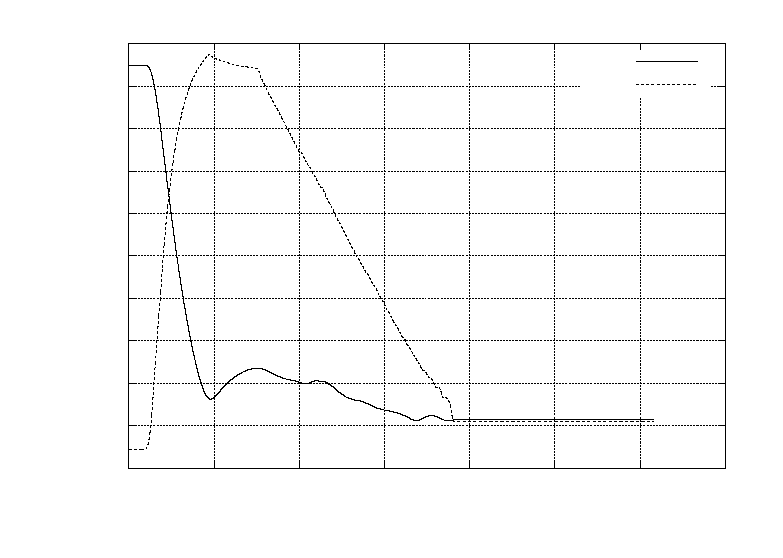
\includegraphics{static_smach_good_plot}}%
    \gplfronttext
  \end{picture}%
\endgroup

    \caption{Fuzzy-controlled static target interception.}\label{f:fuz_stat}
\end{figure}

\begin{figure}
    \centering
    % GNUPLOT: LaTeX picture with Postscript
\begingroup
  \makeatletter
  \providecommand\color[2][]{%
    \GenericError{(gnuplot) \space\space\space\@spaces}{%
      Package color not loaded in conjunction with
      terminal option `colourtext'%
    }{See the gnuplot documentation for explanation.%
    }{Either use 'blacktext' in gnuplot or load the package
      color.sty in LaTeX.}%
    \renewcommand\color[2][]{}%
  }%
  \providecommand\includegraphics[2][]{%
    \GenericError{(gnuplot) \space\space\space\@spaces}{%
      Package graphicx or graphics not loaded%
    }{See the gnuplot documentation for explanation.%
    }{The gnuplot epslatex terminal needs graphicx.sty or graphics.sty.}%
    \renewcommand\includegraphics[2][]{}%
  }%
  \providecommand\rotatebox[2]{#2}%
  \@ifundefined{ifGPcolor}{%
    \newif\ifGPcolor
    \GPcolorfalse
  }{}%
  \@ifundefined{ifGPblacktext}{%
    \newif\ifGPblacktext
    \GPblacktexttrue
  }{}%
  % define a \g@addto@macro without @ in the name:
  \let\gplgaddtomacro\g@addto@macro
  % define empty templates for all commands taking text:
  \gdef\gplbacktext{}%
  \gdef\gplfronttext{}%
  \makeatother
  \ifGPblacktext
    % no textcolor at all
    \def\colorrgb#1{}%
    \def\colorgray#1{}%
  \else
    % gray or color?
    \ifGPcolor
      \def\colorrgb#1{\color[rgb]{#1}}%
      \def\colorgray#1{\color[gray]{#1}}%
      \expandafter\def\csname LTw\endcsname{\color{white}}%
      \expandafter\def\csname LTb\endcsname{\color{black}}%
      \expandafter\def\csname LTa\endcsname{\color{black}}%
      \expandafter\def\csname LT0\endcsname{\color[rgb]{1,0,0}}%
      \expandafter\def\csname LT1\endcsname{\color[rgb]{0,1,0}}%
      \expandafter\def\csname LT2\endcsname{\color[rgb]{0,0,1}}%
      \expandafter\def\csname LT3\endcsname{\color[rgb]{1,0,1}}%
      \expandafter\def\csname LT4\endcsname{\color[rgb]{0,1,1}}%
      \expandafter\def\csname LT5\endcsname{\color[rgb]{1,1,0}}%
      \expandafter\def\csname LT6\endcsname{\color[rgb]{0,0,0}}%
      \expandafter\def\csname LT7\endcsname{\color[rgb]{1,0.3,0}}%
      \expandafter\def\csname LT8\endcsname{\color[rgb]{0.5,0.5,0.5}}%
    \else
      % gray
      \def\colorrgb#1{\color{black}}%
      \def\colorgray#1{\color[gray]{#1}}%
      \expandafter\def\csname LTw\endcsname{\color{white}}%
      \expandafter\def\csname LTb\endcsname{\color{black}}%
      \expandafter\def\csname LTa\endcsname{\color{black}}%
      \expandafter\def\csname LT0\endcsname{\color{black}}%
      \expandafter\def\csname LT1\endcsname{\color{black}}%
      \expandafter\def\csname LT2\endcsname{\color{black}}%
      \expandafter\def\csname LT3\endcsname{\color{black}}%
      \expandafter\def\csname LT4\endcsname{\color{black}}%
      \expandafter\def\csname LT5\endcsname{\color{black}}%
      \expandafter\def\csname LT6\endcsname{\color{black}}%
      \expandafter\def\csname LT7\endcsname{\color{black}}%
      \expandafter\def\csname LT8\endcsname{\color{black}}%
    \fi
  \fi
    \setlength{\unitlength}{0.0500bp}%
    \ifx\gptboxheight\undefined%
      \newlength{\gptboxheight}%
      \newlength{\gptboxwidth}%
      \newsavebox{\gptboxtext}%
    \fi%
    \setlength{\fboxrule}{0.5pt}%
    \setlength{\fboxsep}{1pt}%
\begin{picture}(7200.00,5040.00)%
    \gplgaddtomacro\gplbacktext{%
      \csname LTb\endcsname%
      \put(682,704){\makebox(0,0)[r]{\strut{}$-1$}}%
      \csname LTb\endcsname%
      \put(682,1213){\makebox(0,0)[r]{\strut{}$0$}}%
      \csname LTb\endcsname%
      \put(682,1722){\makebox(0,0)[r]{\strut{}$1$}}%
      \csname LTb\endcsname%
      \put(682,2231){\makebox(0,0)[r]{\strut{}$2$}}%
      \csname LTb\endcsname%
      \put(682,2740){\makebox(0,0)[r]{\strut{}$3$}}%
      \csname LTb\endcsname%
      \put(682,3248){\makebox(0,0)[r]{\strut{}$4$}}%
      \csname LTb\endcsname%
      \put(682,3757){\makebox(0,0)[r]{\strut{}$5$}}%
      \csname LTb\endcsname%
      \put(682,4266){\makebox(0,0)[r]{\strut{}$6$}}%
      \csname LTb\endcsname%
      \put(682,4775){\makebox(0,0)[r]{\strut{}$7$}}%
      \csname LTb\endcsname%
      \put(814,484){\makebox(0,0){\strut{}$0$}}%
      \csname LTb\endcsname%
      \put(2012,484){\makebox(0,0){\strut{}$5$}}%
      \csname LTb\endcsname%
      \put(3210,484){\makebox(0,0){\strut{}$10$}}%
      \csname LTb\endcsname%
      \put(4407,484){\makebox(0,0){\strut{}$15$}}%
      \csname LTb\endcsname%
      \put(5605,484){\makebox(0,0){\strut{}$20$}}%
      \csname LTb\endcsname%
      \put(6803,484){\makebox(0,0){\strut{}$25$}}%
    }%
    \gplgaddtomacro\gplfronttext{%
      \csname LTb\endcsname%
      \put(176,2739){\rotatebox{-270}{\makebox(0,0){\strut{}Error, m}}}%
      \put(3808,154){\makebox(0,0){\strut{}Time, s}}%
      \put(5816,4602){\makebox(0,0)[r]{\strut{}$e_{xy}$}}%
      \put(5816,4382){\makebox(0,0)[r]{\strut{}$e_z$}}%
    }%
    \gplbacktext
    \put(0,0){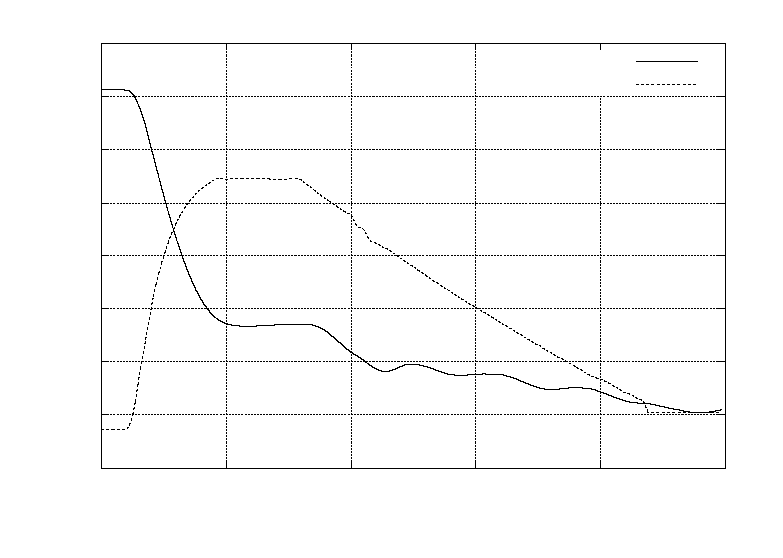
\includegraphics{moving_line_good_plot}}%
    \gplfronttext
  \end{picture}%
\endgroup

    \caption{Fuzzy-controlled dynamic target interception. The target is moving in a straight line with a
    velocity of \SI{0.1}{\meter\per\second}.}\label{f:fuz_dyn}
\end{figure}


%\begin{figure}[ht]
    %\centering
    %\begin{subfigmatrix}{2}
        %\subfigure[Static target interception.\label{f:fuz_stat}]{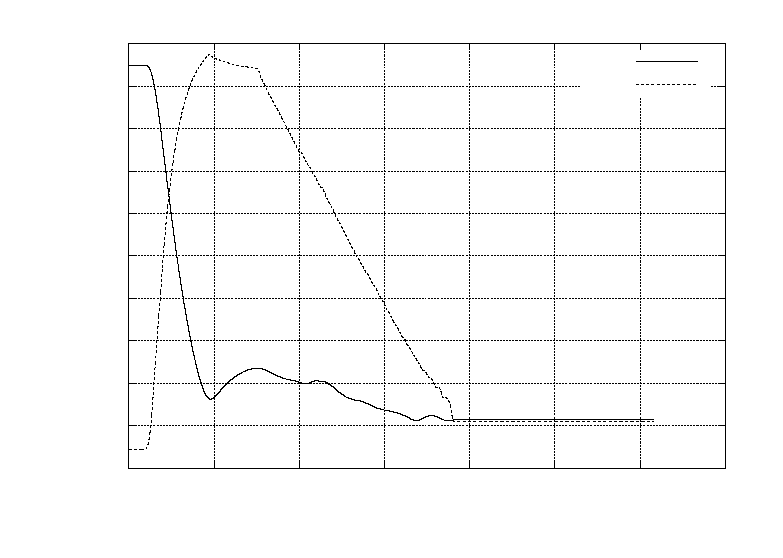
\includegraphics[width=0.49\textwidth]{static_smach_good_plot}}
        %\subfigure[Dynamic target interception.\label{f:fuz_dyn}]{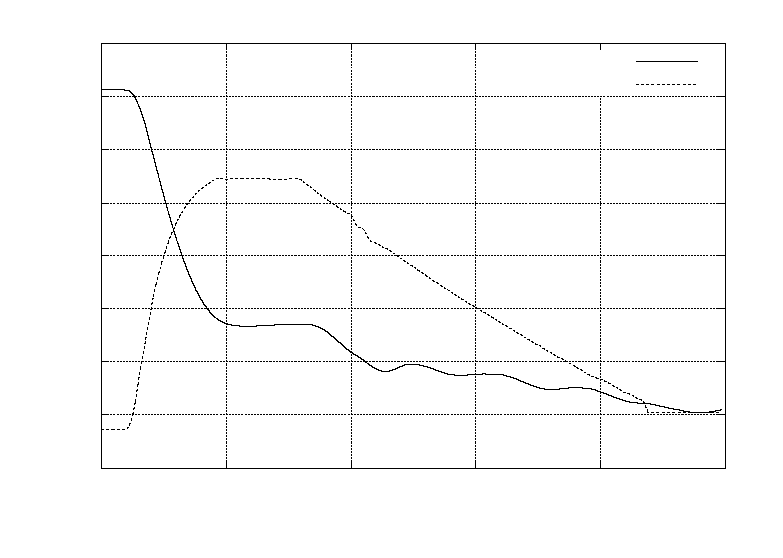
\includegraphics[width=0.49\textwidth]{moving_line_good_plot}}
    %\end{subfigmatrix}
    %\caption{Fuzzy controllers for static and dynamic landing}\label{f:fuzzy_lands}
%\end{figure}


\section{Conclusion}
It has been shown that a pure FLS controller is capable of controlling the position of a multirotor vehicle in
the task of precision landing on a small target. The small size of the platform presents a challenging
landing target; the FLS proved capable enough to overcome this challenge easily. The kalman filtering was an
integral component in providing the controller with a steady estimate of its error state. The components
chosen to accomplish this task are readily available in university laboratory environments and the physical
realization of this system was kept in the forefront of the design process. 

